\let\textcircled=\pgftextcircled
\chapter{Implémentation et Evaluations}
\label{chap:implem_eval}

\initial{C}\textit{e chapitre présente quelques détails d’implémentation et les évaluations que nous avons effectuées pour valider l’intérêt de notre solution.}

\minitoc

\newpage  
\section{Implémentation}
\subsection{Environnement d'implémentation}

\subsubsection{Hyperviseur}

Plusieurs systèmes de virtualisation existent sur le marché. Nous nous sommes donc appuyés sur un certain nombre de critères pour choisir celui que nous allions utiliser dans notre travail. Il s'agit :
\begin{itemize}[label=\ding{43}]
    \item Du \textbf{support para-virtualisation.} La solution que nous proposons concorde avec les principes de la para-virtualisation car elle exige des modifications dans les systèmes d'exploitation invités.
    \item Du \textbf{droit de modification des sources.} L'hyperviseur choisi doit être \textit{open source} afin de pouvoir en obtenir le code source et de pouvoir le modifier sans contrainte.
    \item De la \textbf{communauté informatique travaillant sur le système.} À cause de la documentation disponible et du support à la résolution des bogues.
\end{itemize}
\noindent Sur la base de ces critères, nous avons opté pour l'utilisation de l'hyperviseur \emph{XEN} \cite{article2} car c'est celui qui correspondait le mieux à nos besoins.

\subsubsection{Système d'exploitation}
Les critères de choix du système d'exploitation sont les mêmes que ceux utilisés pour le choix de l'hyperviseur, avec en plus la contrainte de compatibilité entre les deux. Le choix n'a donc pas été difficile, nous avons opté pour le système d'exploitation \emph{Linux} car:
\begin{itemize}[label=\ding{43}]
    \item Linux est le seul système d'exploitation qui supporte la para-virtualisation avec l'hyperviseur Xen;
    \item Linux est \textit{open source} : son code source est disponible et sa modification n'est pas interdite;
    \item Il y a une grande communauté qui travaille sur ce système. En cas de problème, il y a assez de documentations et de forums qui pourront permettre de trouver des solutions aux problèmes rencontrés.
\end{itemize}

\subsubsection{Langage de programmation}
Les mécanismes que nous voulons implémenter nécessitent d'interagir avec le matériel. Il est  donc important d'utiliser un langage de bas niveau. De plus, il s'agit essentiellement de modifier les codes sources de l'hyperviseur et du système d'exploitation, qui sont tous les deux écrits en langage C. C'est la raison pour laquelle nous avons utilisé le C comme langage de programmation.

\subsubsection{Outils de développement}
\paragraph{\textbf{Le compilateur}}
\par\noindent
\par\noindent Le noyau Linux et l'hyperviseur XEN sont écrits dans le langage de programmation C, avec certaines parties du code en langage assembleur. Pour les compiler, il faut utiliser la suite de compilateurs \emph{GCC} (GNU Compiler Collection). GCC est un ensemble de compilateurs créés par le projet GNU \cite{gnu}. GCC est un logiciel libre capable de compiler divers langages de programmation, dont C, C++, Objective-C, Java, Ada et Fortran. \\
On a besoin en outre de l'outil \emph{make} qui est un programme permettant de parcourir le code source et de déterminer quels sont les fichiers qui ont besoin d'être compilés, afin d'appeler le compilateur GCC pour faire le reste du travail.

\paragraph{\textbf{L'éditeur}}
\par\noindent
\par\noindent Lorsqu'on développe sur des projets contenant des millions de lignes de code comme ceux de Linux (environ 16 millions de lignes de code réparties dans 45 mille fichiers) \cite{linux} et XEN (environ 600 mille lignes de code réparties dans 7 mille fichiers), il est nécessaire d'utiliser un bon éditeur pour faciliter la navigation entre les fichiers. Nous avons opté pour les éditeurs \emph{VS Code, Visual Studio Code} et \emph{Sublime Text}.\\

\emph{VS Code} est un éditeur multi-plateforme, \textit{open source} et gratuit supportant une dizaine de langages. C'est un éditeur de code extensible développé par Microsoft pour Windows, Linux et macOS.\\
VS Code combine la simplicité d'un éditeur de code avec ce dont les développeurs ont besoin pour leur cycle de base édition-compilation-débogage. Le code fournit une prise en charge complète de l'édition et du débogage, un modèle d'extensibilité et une intégration légère aux outils existants. Il permet aussi, entre autres fonctionnalités, de retrouver la définition d'une fonction à partir de l'endroit où elle est appelée et de rechercher et remplacer des chaînes de caractères sur la base d'expression régulières.\\
 VS Code est mis à jour tous les mois avec de nouvelles fonctionnalités et corrections de bugs.

\emph{Sublime Text} est un éditeur de texte générique codé en C++ et Python, disponible sur Windows, Mac et Linux. Le logiciel a été conçu tout d'abord comme une extension pour Vim, riche en fonctionnalités. Cet éditeur prend en charge plus de 44 langages de programmation majeurs, et des plugins sont souvent disponibles pour les langages plus rares. Sur son interface graphique, il intègre la plupart des fonctionnalités de base d'un éditeur de texte, dont la coloration syntaxique personnalisable et l’auto complétion. Tout comme VS Code, il permet également de retrouver la définition d'une fonction à partir de l'endroit où elle est appelée et de rechercher et remplacer des chaînes de caractères sur la base d'expression régulières.

\subsection{Détails d'implémentation}
\subsubsection{Définition des hypercalls pour activer et désactiver le PML pour une VM donnée}
Le mécanisme du PML n'est pas activé par défaut, même s'il est supporté par le processeur. Certains hyperviseurs tels que VMWare et XEN ont déjà modifié leur code source pour y intégré ce mécanisme, notamment son activation et son utilisation.\\  XEN dans son code source a intégré le PML, mais uniquement dans le cadre de la migration des machines virtuelles \cite{xen_pml}. En effet, pendant la migration d'une VM, XEN utilise le mécanisme du PML pour traquer les pages chaudes qui doivent être déplacées.\\
Or dans le cadre de notre travail, nous devons être capables d'activer le PML hors de ce contexte, i.e. chaque fois que nous avons besoin d'estimer le WSS d'une VM. Dans XEN, la figure \ref{fig:appel_fonction} présente la file d'appels des fonctions liées à l'activation du PML pour une VM : 
\begin{figure}[H]
    \centering
    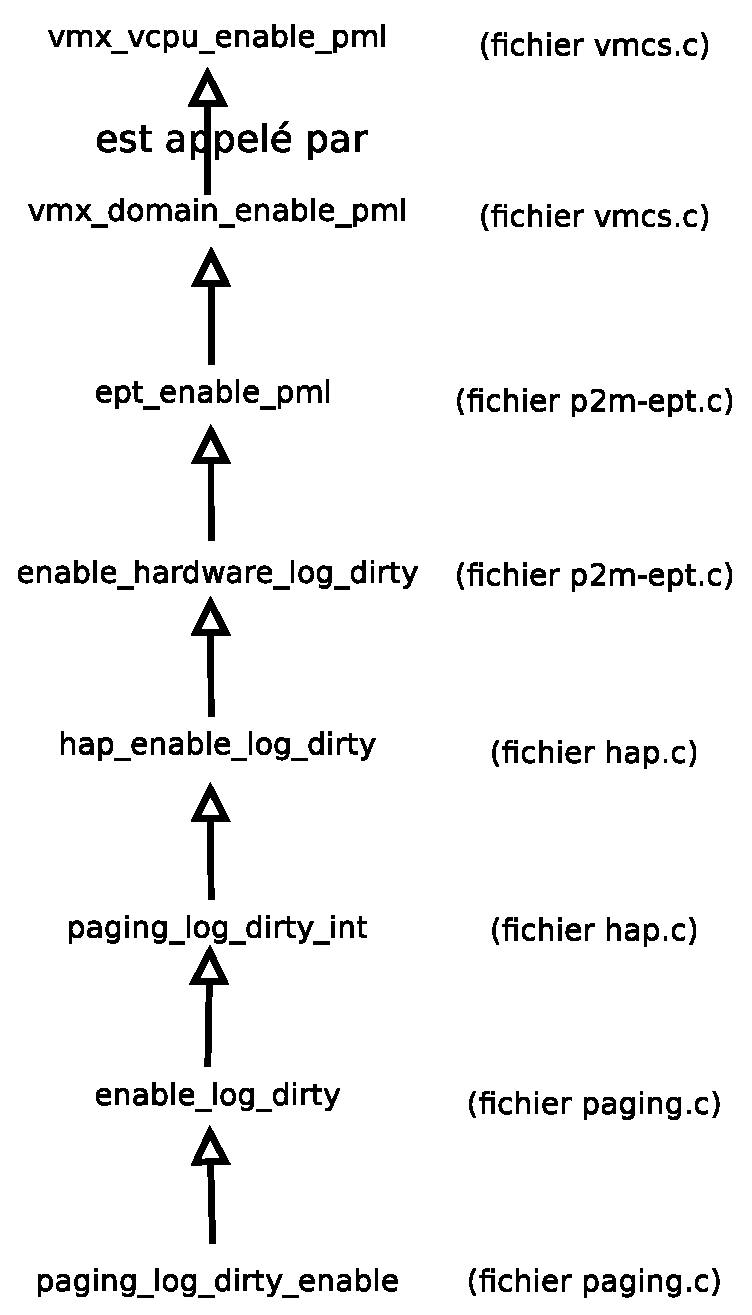
\includegraphics[scale=.6]{chapters/4/fig4/appel_fonction}
    \caption{File d'appels des fonctions liées à l'activation du PML}
    \label{fig:appel_fonction}
\end{figure}

\noindent Comme nous le montre cette file d'appels, le but est d'activer le PML pour les processeurs sur lesquels s'exécutent la VM. Mais tout part de l'activation du mode \textit{log dirty} pour les pages de la VM. C'est ce mode qui va permettre de traquer les pages mémoire utiliser par la machine virtuelle.\\
L'activation du mode \textit{log dirty} dans XEN se fait depuis les tools. Nous avons donc défini des hypercalls à travers les commandes suivantes : $«xl \quad enable-log-dirty» \quad \& \quad  «xl \quad disable-log-dirty»$.

\noindent Un aperçu des lignes de code liées à la définition de ces hypercalls se trouve en annexes \ref{section:enable_disable_logdirty}, codes \ref{lst:enable_logdirty} et \ref{lst:disable_logdirty}.

\subsubsection{Modification de la structure de données bitmap}
\begin{figure}[H]
    \centering
    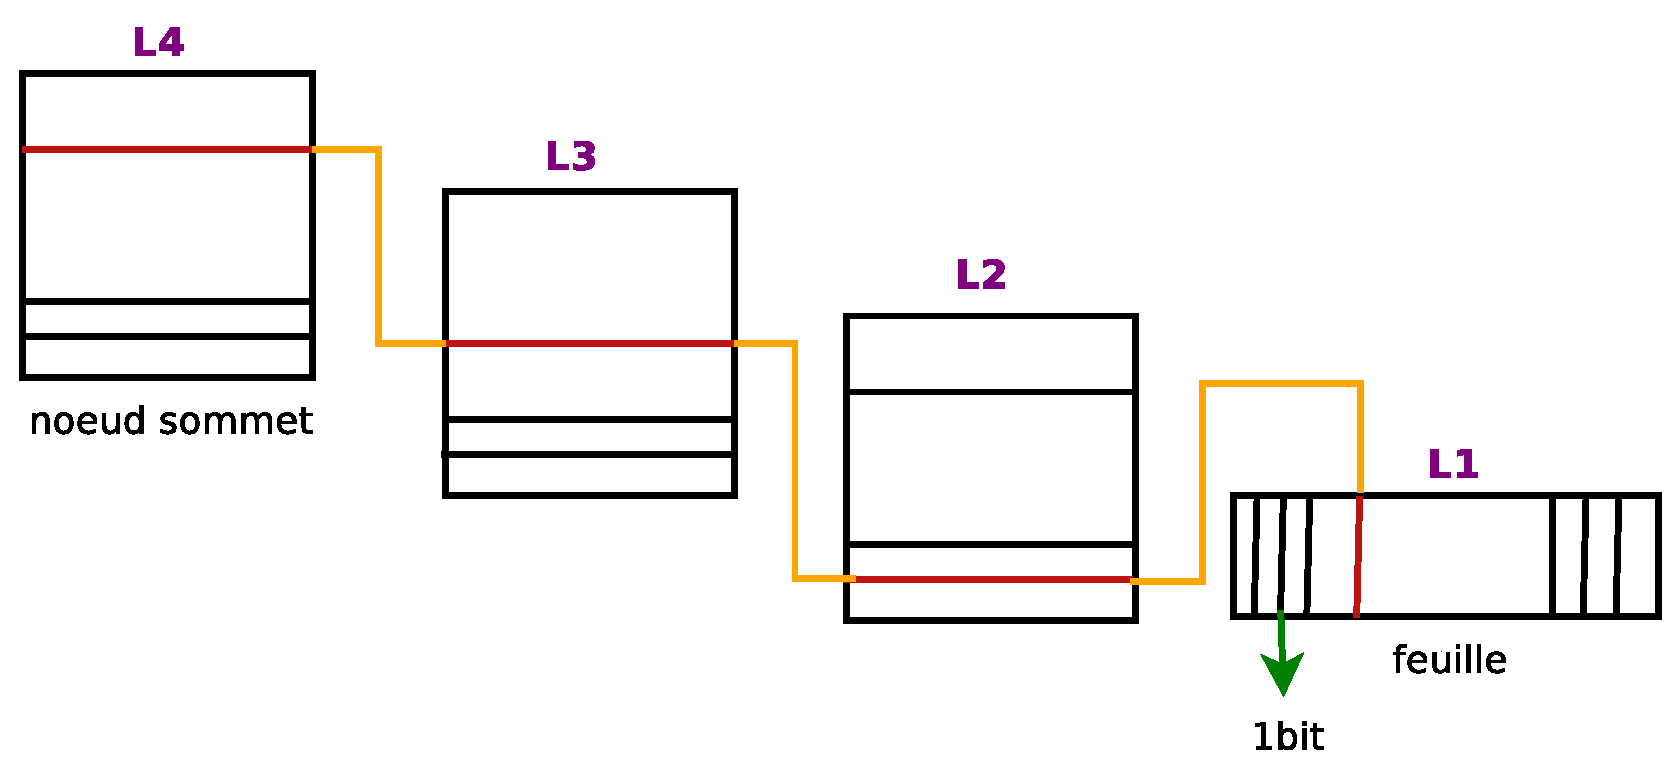
\includegraphics[scale=.6,width=1\linewidth]{chapters/4/fig4/bitmap}
    \caption{Radix tree représentant la bitmap}
    \label{fig:bitmap}
\end{figure}

Actuellement la structure de données qui représente la bitmpa est un \textit{radix tree} dont chaque branche est constituée de 4 niveaux tels que matérialisés par la figure \ref{fig:bitmap}:
\begin{itemize}
    \item 3 noeuds intermédiaires : dans chaque noeud, une entrée est un pointeur vers une entrée dans le noeud suivant.
    \item 1 feuille terminale : ses entrées quant à elle sont des bits dont chacun représente une adresse du log.
\end{itemize}

Chaque noeud de l'arbre est une page de $4Ko$, y compris les feuilles terminales. Étant donné que les entrées d'une feuille sont des bits on peut déterminer le nombre d'entrées dans une feuille. En effet : $$1octet \quad = \quad 2^{3} bits$$ 
$$\Rightarrow 1Ko \quad = \quad 2^{10}*2^{3} bits$$
$$\Rightarrow 4Ko \quad = \quad 2^{2}*2^{10}*2^{3} bits \quad = \quad 2^{15} bits$$
Donc on a $2^{15}$ entrées dans une feuille. Maintenant nous devons garder pour une feuille le même nombre d'entrées mais de type $long$ \footnote{UL : unsigned long} et non plus $bit$. Pour celà nous devons déterminer le nombre $X$ de pages de $4Ko$ dont a besoin pour contenir $2^{15}$ entrées de type $long$ : 
$$X \quad = \quad \frac{taille\_des\_entrees}{taille\_page}$$
$$\quad = \quad \frac{2^{15}*sizeof(UL)}{4Ko}$$
$$ \quad\quad= \quad \frac{2^{15}*sizeof(UL) \footnote{Taille d'un unsigned long}}{2^{2}*2^{10}}$$
$$\quad = \quad 2^{3}*sizeof(UL)$$
$$= \quad 8sizeof(UL)$$

\noindent Sur la base de ces calculs, nous avons rajouté un niveau $L0$. Le \textit{radix tree} est donc modifié de sorte que les entrées du niveau $L1$ actuel soient non plus des bits mais des adresses qui pointent chacune vers une page $L0$, qui elle contiendra les informations loguées i.e. adresses et occurrences.\\

\begin{figure}[H]
    \centering
    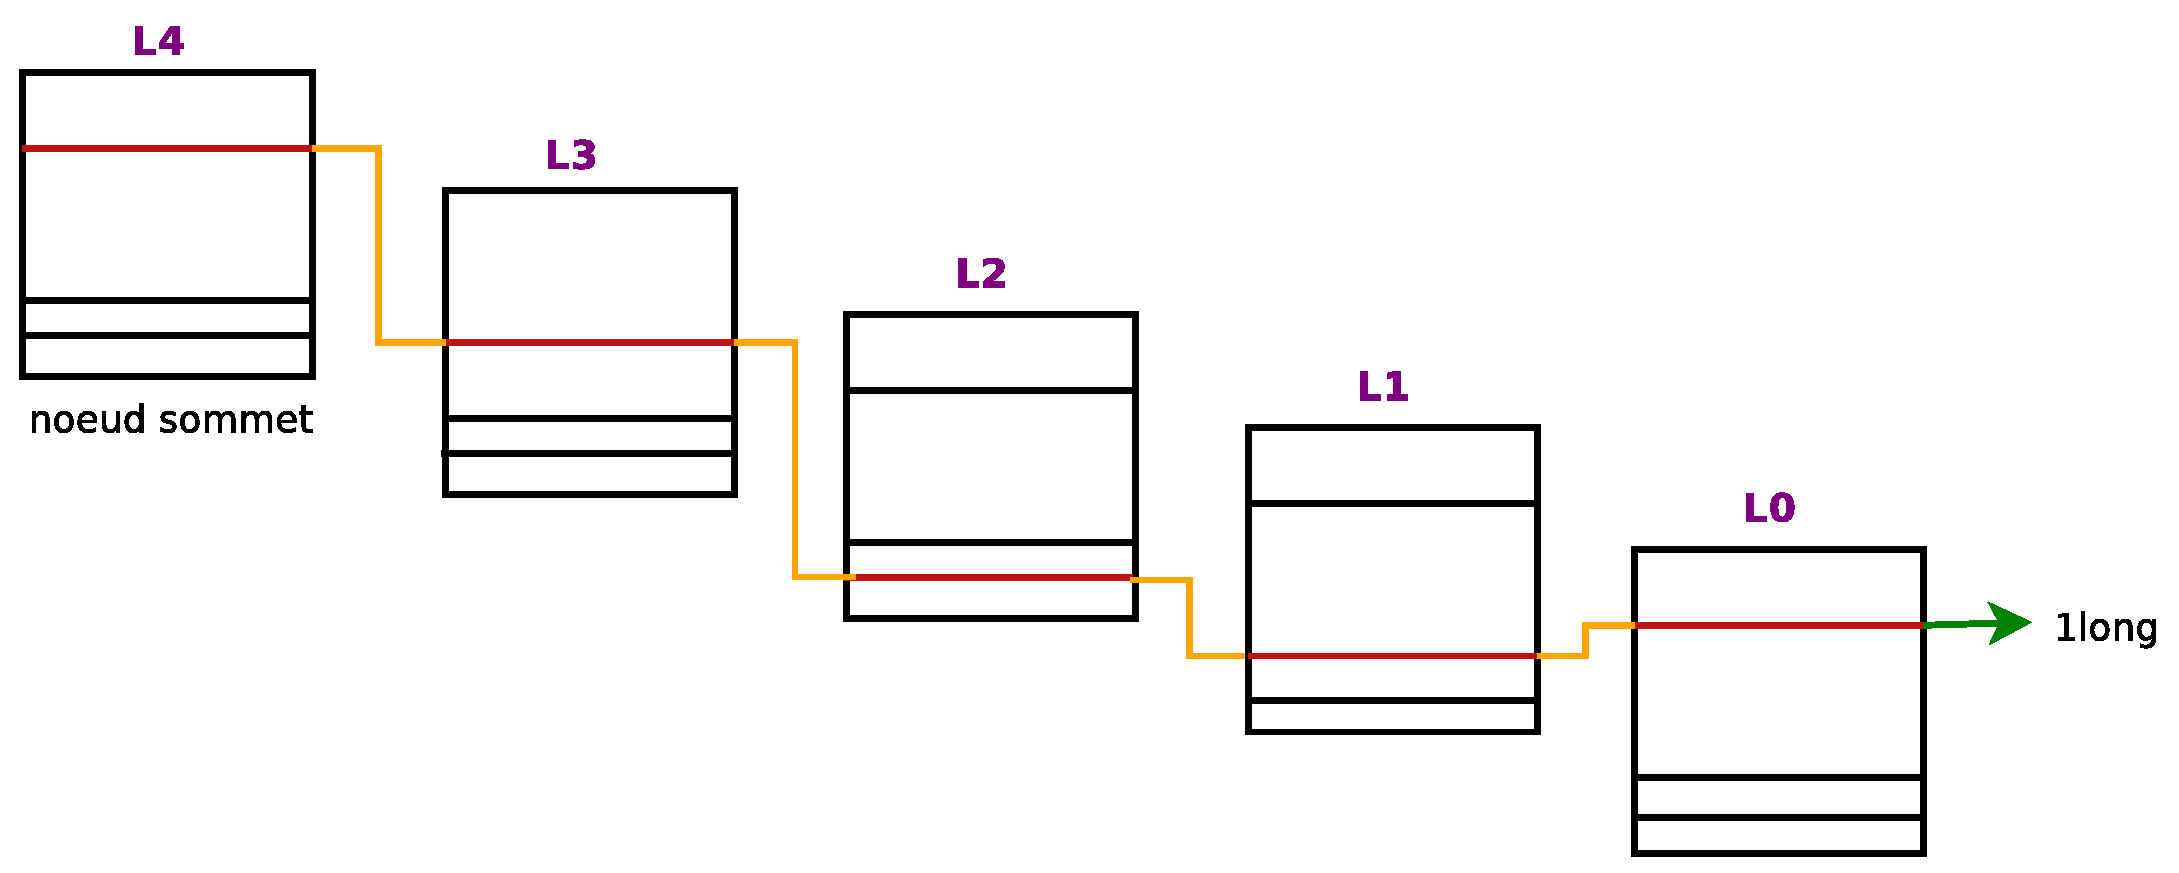
\includegraphics[scale=.6,width=1\linewidth]{chapters/4/fig4/longmap}
    \caption{Radix tree représentant la longmap}
    \label{fig:longmap}
\end{figure}

\noindent La méthode qui permettait de générer une feuille $L1$ a été modifiée telle que présentée dans les codes \ref{lst:leaf_bit} et \ref{lst:leaf_UL} en annexe \ref{section:bitmap}. Et la nouvelle structure est matérialisée par la figure \ref{fig:longmap}.

\subsubsection{Modification du traitant \textit{pml buffer full}}
Nous avons modifié le comportement du mécanisme lorsque le \textit{pml\_log} est plein en accord avec la modification de la structure de consolidation de logs telle que présentée au paragraphe précédent. Ainsi, au moment de vider le buffer, l'algorithme parcours la nouvelle structure de données, et s'il existe déjà une entrée pour l'adresse à enregistrée, son compteur incrémenté. Sinon, une nouvelle entrée est crée et le compteur est initialisé à 1 pour cette adresse.\\
Les modifications effectuées sont dans les codes \ref{lst:pml_buffer_full_avant} et \ref{lst:pml_buffer_full_apres} en annexe \ref{section:pml_buffer_full}.

\subsubsection{Mise en place du mécanisme (hypercall) de copie des logs consolidés de l'hyperviseur vers le dom0}
Pour éviter d'imposer des coûts de surcharge à l'hyperviseur, nous implémentons les algos de calcul dans le dom0. Pour celà, il faut copier les logs depuis la longmap dans l'hyperviseur, vers le dom0 (figure \ref{fig:collect-dirty-logs}). Ceci ne peut se faire qu'à l'aide d'un hypercall que nous avons donc défini : $«xl \quad collect-dirty-logs»$.

\begin{figure}[H]
    \centering
    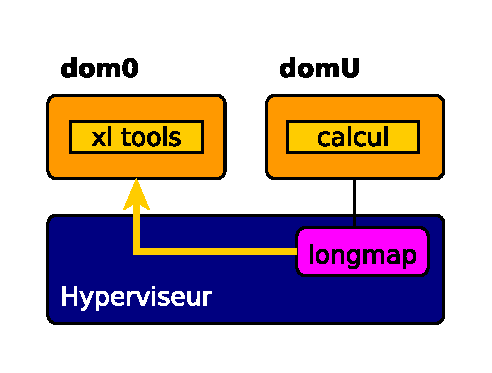
\includegraphics[scale=.8]{chapters/4/fig4/collect-dirty-logs}
    \caption{Copie des logs de l'hyperviseur vers le dom0}
    \label{fig:collect-dirty-logs}
\end{figure}

\noindent Cet hypercall est appelé avec l'$id$ de la VM en paramètre. Ainsi, dès qu'on fait un $xl \quad collect-dirty-logs \quad id\_vm$, la chaîne d'appel de fonctions de l'hypercall  est la suivante :
\begin{figure}[H]
    \centering
    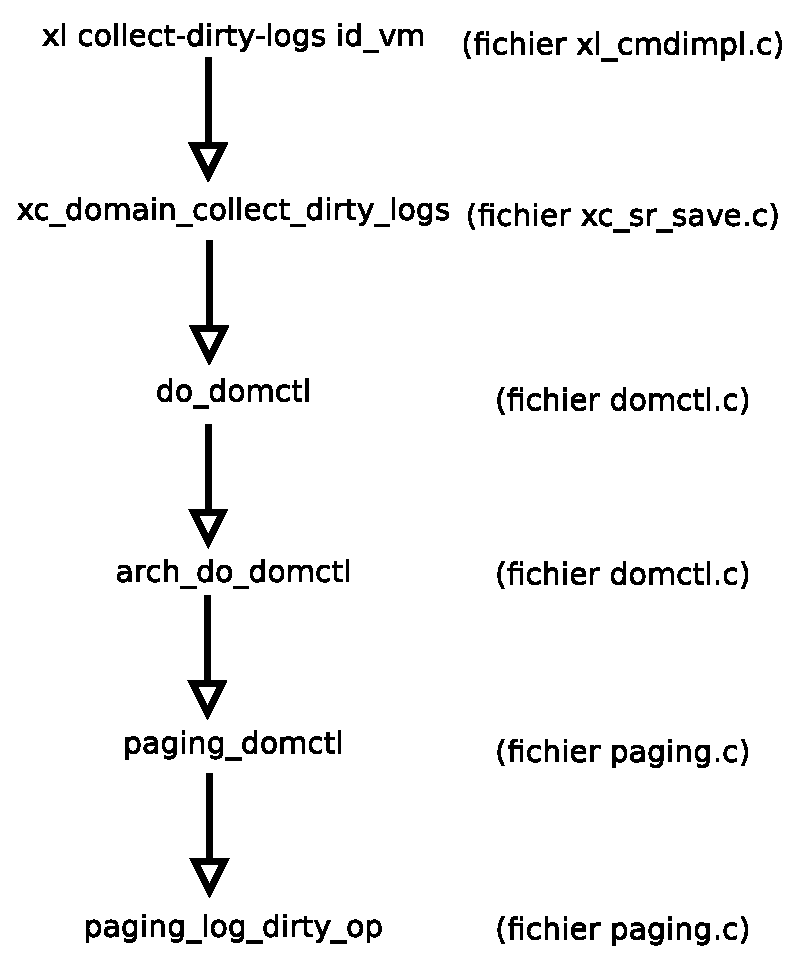
\includegraphics[scale=.6]{chapters/4/fig4/collect-dirty-logs_appel_fonction}
    \caption{Copie des logs de l'hyperviseur vers le dom0 : chaîne d'appel de fonctions}
    \label{fig:collect-dirty-logs_appel_fonction}
\end{figure}

\noindent Cette dernière méthode $paging\_log\_dirty\_op$ , nous l'avons modifiée pour remonter les logs vers le dom0. L'algorithme implémenté dans cette méthode consiste à copier dans les logs de XEN, le contenu de la $longmap$ et compter le nombre total de pages différentes.\\
La définition de la commande $xl$ pour la collecte est en annexe \ref{section:copie_logs}, code \ref{lst:xl}, et celle  de la fonction $xc\_domain\_collect\_dirty\_logs$ code \ref{fig:xc_domain_collect_dirty_logs}.

\subsubsection{Implémentation de la version 0 de l'algorithme d'estimation du WSS}
Enfin, nous avons implémenter une première version de l'algorithme que nous présentons au chapitre précédent. Cette version ne prend en compte que les parties de l'architecture proposée que nous avons pu implémenter, les autres nécessitant une modification du matériel (modification du processeur).\\
Nous avons écrit un script (voir code \ref{lst:script_collect}) qui permet de collecter les logs d'une VM sur une période $T$, ceci toutes $x$ les secondes ($T$ et $x$ donnés en paramètre du script). Le script trace au fur et à mesure de la collecte, une courbe représentant la variation du nombre total d'adresses enregistrées en fonction du temps. Lorsque cette variation se stabilise, i.e. lorsque la courbe devient constante, l'algorithme s'arrête et l'estimation est faite. \\
Des exemples d'application de cet algorithme et des graphes générés sont présentés ci-après dans la section \textit{Évaluations}.

\section{Évaluations}

\subsection{Environnement d'évaluation}
Les expérimentations que nous avons menées ont nécessité l'utilisation d'un seul serveur physique. Les caractéristiques de la machine hôte sont regroupées dans le tableau \ref{table:caracteristiques_machines} suivant.
\begin{table}[H]
  \begin{center}
    \caption{Caractéristiques de la machine physique dans les expérimentations}
    \begin{tabular}{|>{\bfseries}l|c|}
      \hline
      \cellcolor[RGB]{165,42,42}\textcolor{white}{\textbf{Caractéristique}} & \cellcolor[RGB]{165,42,42}\textcolor{white}{\textbf{Valeur}}\\
      \hline
      \hline
      Fabricant & Dell Inc \\ \hline
      Famille de processeur & Intel(R) Core(TM) i7-7600U \\ \hline
      Architecture du processeur & x86\_64 \\ \hline
      Nombre de CPUs & 4 \\ \hline
      Nombre de cœurs par CPU & 2 \\ \hline
      Fréquence des cœurs & 2,80GHz \\ \hline
      Taille de la RAM & 16Go \\ \hline
    \end{tabular}
    \label{tab:caracteristiques_machines}
  \end{center}
\end{table}

\noindent Nous avons effectué les expérimentations avec des charges de travail synthétiques. 

\begin{figure*}
  \centering
  \scriptsize
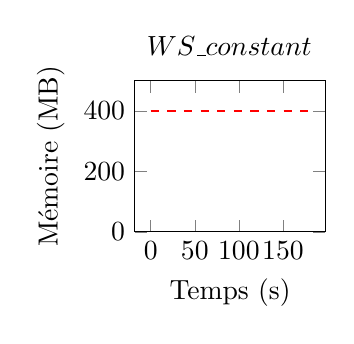
\begin{tikzpicture}
 \begin{axis}[
    name=mygraph,
    height=3.5cm,
    width=4cm,
    legend style={at={(0.5,1.45)},
    anchor=north,legend columns=-1},
    ymax=500,
    ymin=0,
  %legend cell align=left,
    ylabel near ticks,
    ylabel={Mémoire (MB)},
    xlabel={Temps (s)},
  ]%[name path=A]
   \addplot [red,dashed,line width=1pt] coordinates {
    (0,400) (180,400)
  };
%  \legend{$W_1$}
\end{axis}
\node[anchor=north] at (1.2,2.6) {$WS\_constant$};
\end{tikzpicture}
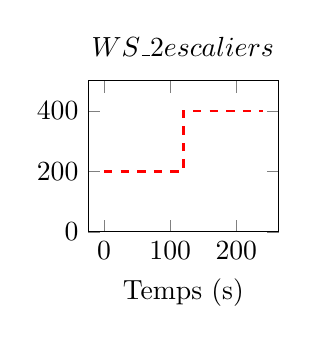
\begin{tikzpicture}
 \begin{axis}[
     name=mygraph,
     height=3.5cm,
     width=4cm,
     legend style={at={(0.5,1.45)},
     anchor=north,legend columns=-1},
     ymax=500,
     ymin=0,
  %legend cell align=left,
    ylabel near ticks,
    xlabel={Temps (s)},
  ]%[name path=A]
   \addplot [red,dashed,line width=1pt] coordinates {
    (0,200) (120,200) (120,400) (240,400)
   };
 \end{axis}
\node[anchor=north] at (1.2,2.6) {$WS\_2escaliers$};
\end{tikzpicture}
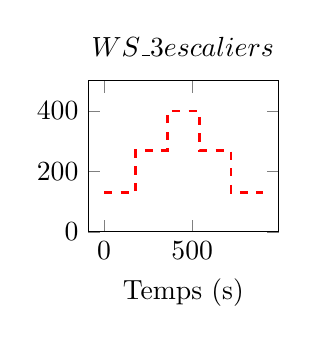
\begin{tikzpicture}
 \begin{axis}[
     name=mygraph,
     height=3.5cm,
     width=4cm,
     legend style={at={(0.5,1.45)},
     anchor=north,legend columns=-1},
     ymax=500,
     ymin=0,
  %legend cell align=left,
     ylabel near ticks,
     xlabel={Temps (s)},
  ]%[name path=A]
   \addplot [red,dashed,line width=1pt] coordinates {
     (0,130) (180,130) (180,270) (360,270) (360,400) (540,400) (540,270) (720,270) (720,130) (900,130)  
  };
\end{axis}
\node[anchor=north] at (1.2,2.6) {$WS\_3escaliers$};
\end{tikzpicture}
\caption{Ensemble des charges de travail synthétiques}
\label{fig:set_workloads}
\end{figure*}

\noindent La figure \ref{fig:set_workloads} présente pour chacune des charges, la variation attendue du WSS en fonction du temps. Nous avons exécuté dans la VM des applications qui manipulent toutes un working set de $400MB$ (soit $400*1024/4 \quad = \quad 102400$ pages méoire), mais avec de façons différentes : utilisation constante et variation en escaliers.\\
Pour chacune des expérimentations ci-après, nous allons présenter les résultats obtenus avec les solutions existantes et ensuite avec la solution que nous avons implémentée.

\subsection{Expérimentation 1 : charge synthétique manipulant un working set constant}

\noindent Comme nous pouvons le voir sur la figure \ref{fig:eval_pml_cst}, la technique que nous avons mise sur pied détecte $105000$ pages, soit $410MB$ comme valeur estimée du \emph{working set}, pour un programme manipulant $102400$ pages.\\

\begin{figure}[H]
  \centering  
  \scriptsize
%%%%%%%%%%%%%%%%%%%%%Xen Self-ballooning Line 1 Column 1
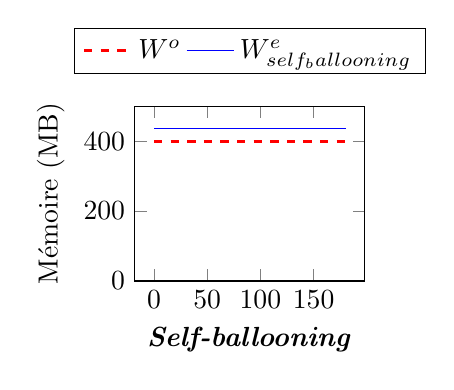
\begin{tikzpicture}
 \begin{axis}[
        height=3.8cm,
        width=4.5cm,
        legend style={at={(0.5,1.45)},
        anchor=north,
        legend columns=-1},       
        ymax=500,
        ymin=0,
  %legend cell align=left, 
        ylabel near ticks,
        ylabel style={align=center}, 
        ylabel={Mémoire (MB)},
        xlabel={\textbf{{\em Self-ballooning}}},
  ]%[name path=A]
   \addplot [red,dashed,line width=1pt] coordinates {
    (0,400) (180,400)
  };  
   \addplot [blue] coordinates {
    (0,437) (180,437)
  }; 
  \legend{$W^o$,$W^{e}_{self_ballooning}$}    
\end{axis}  
\end{tikzpicture}
%%%%%%%%%%%%%%%%%%%%%
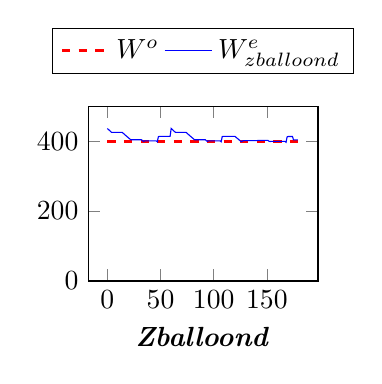
\begin{tikzpicture}
 \begin{axis}[
        height=3.8cm,
        width=4.5cm,
        legend style={at={(0.5,1.45)},
        anchor=north,legend columns=-1},        
        ymax=500,
        ymin=0,
  %legend cell align=left, 
        %ylabel near ticks,
        ylabel style={align=center}, 
        xlabel={\textbf{{\em Zballoond}}},
  ]%[name path=A]
   \addplot [red,dashed,line width=1pt] coordinates {  
      (0,400) (180,400)
   };
   \addplot [blue] coordinates {
    (0,436.5625) (1,433.7109375) (2,430.88671875) (3,428.08984375) (4,425.32421875) (5,425.33203125) (6,425.33203125) (7,425.33203125) (8,425.33203125) (9,425.33203125) (10,425.33203125) (11,425.33203125) (12,425.33203125) (13,425.33203125) (14,425.33203125) (15,422.59375) (16,419.8828125) (17,417.19921875) (18,414.5390625) (19,411.90625) (20,409.30078125) (21,406.72265625) (22,404.16796875) (23,404.32421875) (24,404.32421875) (25,404.32421875) (26,404.32421875) (27,404.32421875) (28,404.32421875) (29,404.32421875) (30,404.32421875) (31,404.32421875) (32,404.32421875) (33,401.79296875) (34,399.2890625) (35,400.875) (36,400.8828125) (37,400.8828125) (38,400.91796875) (39,400.91796875) (40,400.91796875) (41,400.91796875) (42,400.91796875) (43,400.91796875) (44,400.91796875) (45,400.91796875) (46,400.91796875) (47,398.421875) (48,413.15234375) (49,413.78125) (50,413.78125) (51,413.81640625) (52,413.81640625) (53,413.81640625) (54,413.81640625) (55,413.81640625) (56,413.81640625) (57,413.81640625) (58,413.81640625) (59,413.81640625) (60,436.5625) (61,433.7109375) (62,430.88671875) (63,428.08984375) (64,425.32421875) (65,425.33203125) (66,425.33203125) (67,425.33203125) (68,425.33203125) (69,425.33203125) (70,425.33203125) (71,425.33203125) (72,425.33203125) (73,425.33203125) (74,425.33203125) (75,422.59375) (76,419.8828125) (77,417.19921875) (78,414.5390625) (79,411.90625) (80,409.30078125) (81,406.72265625) (82,404.16796875) (83,404.32421875) (84,404.32421875) (85,404.32421875) (86,404.32421875) (87,404.32421875) (88,404.32421875) (89,404.32421875) (90,404.32421875) (91,404.32421875) (92,404.32421875) (93,401.79296875) (94,399.2890625) (95,400.875) (96,400.8828125) (97,400.8828125) (98,400.91796875) (99,400.91796875) (100,400.91796875) (101,400.91796875) (102,400.91796875) (103,400.91796875) (104,400.91796875) (105,400.91796875) (106,400.91796875) (107,398.421875) (108,413.15234375) (109,413.78125) (110,413.78125) (111,413.81640625) (112,413.81640625) (113,413.81640625) (114,413.81640625) (115,413.81640625) (116,413.81640625) (117,413.81640625) (118,413.81640625) (119,413.81640625) (120,413.81640625) (121,411.19140625) (122,408.59375) (123,406.01953125) (124,403.47265625) (125,400.953125) (126,398.45703125) (127,400.28515625) (128,401.6875) (129,401.6953125) (130,401.6953125) (131,401.73046875) (132,401.73046875) (133,401.73046875) (134,401.73046875) (135,401.73046875) (136,401.73046875) (137,401.73046875) (138,401.73046875) (139,401.73046875) (140,401.73046875) (141,401.83203125) (142,402.37109375) (143,402.37109375) (144,402.37109375) (145,402.37109375) (146,402.37109375) (147,402.37109375) (148,402.37109375) (149,402.37109375) (150,402.37109375) (151,402.37109375) (152,399.859375) (153,399.23828125) (154,399.45703125) (155,399.4921875) (156,399.4921875) (157,399.4921875) (158,399.49609375) (159,399.49609375) (160,399.49609375) (161,399.49609375) (162,399.49609375) (163,399.49609375) (164,399.49609375) (165,399.49609375) (166,399.49609375) (167,399.49609375) (168,397.015625) (169,412.4609375) (170,413.5546875) (171,413.5546875) (172,413.5546875) (173,413.5546875) (174,413.5546875) (175,403.7890625) (176,403.7890625) (177,403.7890625) (178,403.7890625) (179,403.7890625)
  };
  \legend{$W^o$,$W^{e}_{zballoond}$}        
\end{axis}  
\end{tikzpicture}
 %%%%%%%%%%%%%%%%%%%%%
 \begin{tikzpicture}
 \begin{axis}[
        height=3.8cm,
        width=4.5cm,
        legend style={at={(0.5,1.45)},
        anchor=north,legend columns=-1},        
        ymax=600,
        ymin=0,
  %legend cell align=left, 
        %ylabel near ticks,
        ylabel style={align=center}, 
        xlabel={\textbf{{\em VMware}}},
  ]%[name path=A] 
  \addplot [red,dashed,line width=1pt] coordinates {
    (0,400) (180,400)
  };  
   \addplot [blue] coordinates {
    (12.8571428571,365) (25.7142857142,408) (38.5714285713,448) (51.4285714284,493) (64.2857142855,417) (77.1428571426,445) (89.9999999997,490) (102.8571428568,443) (115.7142857139,494) (128.571428571,440) (141.4285714281,477) (154.2857142852,536) (167.1428571423,406) (179.9999999994,442)
  };    
  \legend{$W^o_$,$W^e_{vmware}$}        
\end{axis}  
\end{tikzpicture}
 %%%%%%%%%%%%%%%%%%%%%%%%%%%%%%%%%%%%%%%%
 \begin{tikzpicture}
 \begin{axis}[
        height=3.8cm,
        width=4.5cm,
        legend style={at={(0.5,1.45)},
        anchor=north,legend columns=-1},        
        ymax=500,
        ymin=0,
  %legend cell align=left, 
        %ylabel near ticks,
        ylabel style={align=center}, 
        xlabel={\textbf{{\em Geiger}}},
  ]%[name path=A] 
  \addplot [red,dashed,line width=1pt] coordinates {
    (0,400) (180,400)
  };  
   \addplot [blue] coordinates {
    (0,400) (180,400)
  };   
  \legend{$W^o_$,$W^e_{geiger}$}         
\end{axis}  
\end{tikzpicture}
 %%%%%%%%%%%%%%%%%%%%%%%%%%%%%%%%%%%%%%%%%
 \begin{tikzpicture}
 \begin{axis}[
          height=3.8cm,
          width=4.5cm,
          legend style={at={(0.5,1.45)},
          anchor=north,legend columns=-1},        
          ymax=500,
          ymin=0,
          %legend cell align=left, 
          %ylabel near ticks,
          ylabel style={align=center}, xlabel={\textbf{{\em Exclusive-Cache}}},
  ]%[name path=A] 
  \addplot [red,dashed,line width=1pt] coordinates {
    (0,400) (180,400)
  };    
   \addplot [blue] coordinates {
    (0,400) (180,400)
  };   
  \legend{$W^o_$,$W^e_{cache}$}         
\end{axis}  
\end{tikzpicture}
\caption{Résultats d'évaluations de la première charge synthétique avec les techniques existantes\\ \centering\bf $W^o$ : WSS escompté -- $W^e$ : WSS estimé}
\label{fig:studied_technique_ws_cst}
\end{figure}

L'application qui tourne dans la VM utilise activement les $102400$ pages qui constituent son \emph{working set}. Le surplus observé trouve son explication au paragraphe \ref{subsubsection:limites_pml_actuel} - \textit{limite 4}. En effet, comme nous l'avons expliqué les pages de la table de pages sont également loguées pendant le mécanisme, et celles-ci ne sont pas prises en compte dans la valeur expérimentale de la mémoire utilisée par l'application.

\begin{figure}[H]
  \centering  
  \scriptsize
%%%%%%%%%%%%%%%%%%%%%Xen Self-ballooning Line 1 Column 1
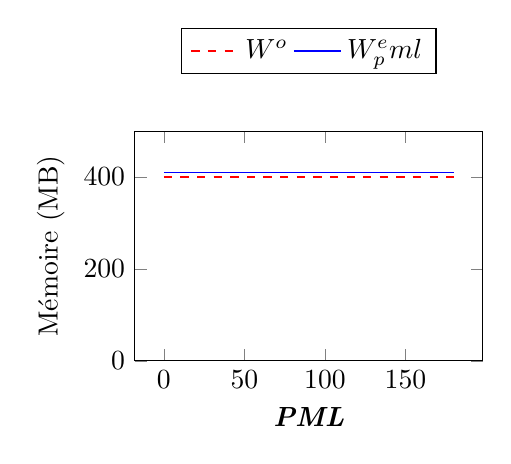
\begin{tikzpicture}
  \begin{axis}[
        height=4.5cm,
        width=6cm,
        legend style={at={(0.5,1.45)},
        anchor=north,
        legend columns=-1},       
        ymax=500,
        ymin=0,
  %legend cell align=left, 
        ylabel near ticks,
        ylabel style={align=center}, 
        ylabel={Mémoire (MB)},
        xlabel={\textbf{{\em PML}}},
  ]%[name path=A]
   \addplot [red,dashed,line width=1pt] coordinates {
        (0,400) (180,400)
   };  
   \addplot [blue] coordinates {
        (0,410) (180,410)
    }; 
  \legend{$W^o$,$W^{e}_pml$}    
\end{axis}  
\end{tikzpicture}
\caption{Résultats d'évaluations de la première charge synthétique avec la technique implémentée. $W^o$ : WSS escompté -- $W^e$ WSS : estimé}
\label{fig:eval_pml_cst}
\end{figure}

\subsection{Expérimentation 2 : charges synthétiques manipulant un working set variable (en escaliers)}
En observant les résultats présentés à la figure \ref{fig:studied_technique_ws_var}, on constate que pour la plus part des techniques existantes il est difficile de détecter les variations de mémoire. A l'opposé, la technique que nous avons implémentée, dont les résultats sont présentés à la figure \ref{fig:eval_pml_var}.\\
\par

\begin{figure}[H]
  \centering
  \scriptsize
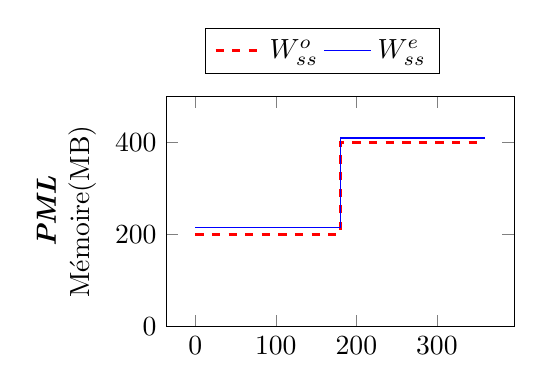
\begin{tikzpicture}
 \begin{axis}[
      %name=mygraph,
        height=4.5cm,
        width=6cm,
        legend style={at={(0.45,1.3)},
        anchor=north,legend columns=-1},        
        ymax=500,
        ymin=0,
  %legend cell align=left, 
        ylabel near ticks,
        ylabel style={align=center},
        ylabel={\textbf{{\em PML}}\\Mémoire(MB)},
  ]%[name path=A]
  \addplot [red,dashed,line width=1pt] coordinates {
    (0,200) (180,200) (180,400) (360,400)
  };
  \addplot [blue] coordinates {
    (0,216) (180,216) (180,410) (360,410)
  };
\legend{$W^o_{ss}$,$W^{e}_{ss}$}  
\end{axis}
%\node[anchor=north] at (1.2,2.6) {$WS\_constant$};
\end{tikzpicture}
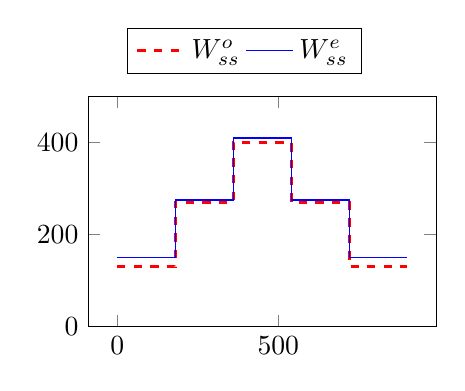
\begin{tikzpicture}
 \begin{axis}[
        height=4.5cm,
        width=6cm,
        legend style={at={(0.45,1.3)},
        anchor=north,legend columns=-1},        
        ymax=500,
        ymin=0,
  %legend cell align=left, 
        ylabel near ticks,
  ]%[name path=A]
   \addplot [red,dashed,line width=1pt] coordinates {
     (0,130) (180,130) (180,270) (360,270) (360,400) (540,400) (540,270) (720,270) (720,130) (900,130) 
  };
  \addplot [blue] coordinates {
     (0,150) (180,150) (180,275) (360,275) (360,410) (540,410) (540,275) (720,275) (720,150) (900,150) 
  };
\legend{$W^o_{ss}$,$W^{e}_{ss}$} 
 \end{axis}
%\node[anchor=north] at (1.2,2.6) {$WS\_2escaliers$};
\end{tikzpicture}\caption{Résultats d'évaluations des charges variables avec le PML. $W^o_{ss}$ : WSS escompté -- $W^e_{ss}$ WSS : estimé}
\label{fig:eval_pml_var}
\end{figure}

\begin{figure}
   
   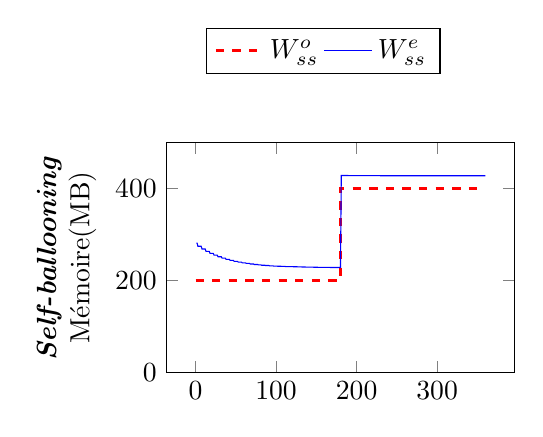
\begin{tikzpicture}
  \begin{axis}[
        %name=mygraph,
        height=4.5cm,
        width=6cm,
        legend style={at={(0.45,1.5)},
        anchor=north,legend columns=-1},        
        ymax=500,
        ymin=0,
  %legend cell align=left, 
        ylabel near ticks,
        ylabel style={align=center},
        ylabel={\textbf{{\em Self-ballooning}}\\Mémoire(MB)},
  ]%[name path=A]
  \addplot [red,dashed,line width=1pt] coordinates {
    (0,200) (180,200) (180,400) (360,400)
  }; 
  \addplot [blue] coordinates {
    (1,281.09375) (2,281.09375) (3,274.40234375) (4,274.40234375) (5,274.40234375) (6,274.40234375) (7,274.40234375) (8,268.546875) (9,268.546875) (10,268.546875) (11,268.546875) (12,268.546875) (13,263.421875) (14,263.421875) (15,263.421875) (16,263.421875) (17,263.421875) (18,258.94140625) (19,258.94140625) (20,258.94140625) (21,258.94140625) (22,258.94140625) (23,255.0234375) (24,255.0234375) (25,255.0234375) (26,255.0234375) (27,255.0234375) (28,251.59375) (29,251.59375) (30,251.59375) (31,251.59375) (32,251.59375) (33,248.59375) (34,248.59375) (35,248.59375) (36,248.59375) (37,248.59375) (38,245.96875) (39,245.96875) (40,245.96875) (41,245.96875) (42,245.96875) (43,243.671875) (44,243.671875) (45,243.671875) (46,243.671875) (47,243.671875) (48,241.66015625) (49,241.66015625) (50,241.66015625) (51,241.66015625) (52,241.66015625) (53,239.90234375) (54,239.90234375) (55,239.90234375) (56,239.90234375) (57,239.90234375) (58,238.36328125) (59,238.36328125) (60,238.36328125) (61,238.36328125) (62,238.36328125) (63,237.015625) (64,237.015625) (65,237.015625) (66,237.015625) (67,237.015625) (68,235.8359375) (69,235.8359375) (70,235.8359375) (71,235.8359375) (72,235.8359375) (73,234.8046875) (74,234.8046875) (75,234.8046875) (76,234.8046875) (77,234.8046875) (78,233.90234375) (79,233.90234375) (80,233.90234375) (81,233.90234375) (82,233.11328125) (83,233.11328125) (84,233.11328125) (85,233.11328125) (86,233.11328125) (87,232.421875) (88,232.421875) (89,232.421875) (90,232.421875) (91,232.421875) (92,231.81640625) (93,231.81640625) (94,231.81640625) (95,231.81640625) (96,231.81640625) (97,231.2890625) (98,231.2890625) (99,231.2890625) (100,231.2890625) (101,231.2890625) (102,230.82421875) (103,230.82421875) (104,230.82421875) (105,230.82421875) (106,230.82421875) (107,230.5) (108,230.5) (109,230.5) (110,230.5) (111,230.5) (112,230.21875) (113,230.21875) (114,230.21875) (115,230.21875) (116,230.21875) (117,229.97265625) (118,229.97265625) (119,229.97265625) (120,229.97265625) (121,229.97265625) (122,229.75390625) (123,229.75390625) (124,229.75390625) (125,229.75390625) (126,229.75390625) (127,229.5625) (128,229.5625) (129,229.5625) (130,229.5625) (131,229.5625) (132,229.31640625) (133,229.31640625) (134,229.31640625) (135,229.31640625) (136,229.31640625) (137,229.1015625) (138,229.1015625) (139,229.1015625) (140,229.1015625) (141,229.1015625) (142,228.9140625) (143,228.9140625) (144,228.9140625) (145,228.9140625) (146,228.9140625) (147,228.75) (148,228.75) (149,228.75) (150,228.75) (151,228.75) (152,228.60546875) (153,228.60546875) (154,228.60546875) (155,228.60546875) (156,228.60546875) (157,228.48046875) (158,228.48046875) (159,228.48046875) (160,228.48046875) (161,228.48046875) (162,228.37109375) (163,228.37109375) (164,228.37109375) (165,228.37109375) (166,228.37109375) (167,228.2734375) (168,228.2734375) (169,228.2734375) (170,228.2734375) (171,228.2734375) (172,228.1875) (173,228.1875) (174,228.1875) (175,228.1875) (176,228.1875) (177,228.11328125) (178,228.11328125) (179,228.11328125) (180,228.11328125) (181,428.359375) (182,428.359375) (183,428.359375) (184,428.359375) (185,428.28515625) (186,428.28515625) (187,428.28515625) (188,428.28515625) (189,428.28515625) (190,428.21875) (191,428.21875) (192,428.21875) (193,428.21875) (194,428.21875) (195,428.16015625) (196,428.16015625) (197,428.16015625) (198,428.16015625) (199,428.16015625) (200,428.109375) (201,428.109375) (202,428.109375) (203,428.109375) (204,428.109375) (205,428.06640625) (206,428.06640625) (207,428.06640625) (208,428.06640625) (209,428.06640625) (210,428.02734375) (211,428.02734375) (212,428.02734375) (213,428.02734375) (214,428.02734375) (215,427.9921875) (216,427.9921875) (217,427.9921875) (218,427.9921875) (219,427.9921875) (220,427.9609375) (221,427.9609375) (222,427.9609375) (223,427.9609375) (224,427.9609375) (225,427.93359375) (226,427.93359375) (227,427.93359375) (228,427.93359375) (229,427.93359375) (230,427.91015625) (231,427.91015625) (232,427.91015625) (233,427.91015625) (234,427.91015625) (235,427.890625) (236,427.890625) (237,427.890625) (238,427.890625) (239,427.890625) (240,427.875) (241,427.875) (242,427.875) (243,427.875) (244,427.875) (245,427.859375) (246,427.859375) (247,427.859375) (248,427.859375) (249,427.84765625) (250,427.84765625) (251,427.84765625) (252,427.84765625) (253,427.84765625) (254,427.8359375) (255,427.8359375) (256,427.8359375) (257,427.8359375) (258,427.8359375) (259,427.82421875) (260,427.82421875) (261,427.82421875) (262,427.82421875) (263,427.82421875) (264,427.81640625) (265,427.81640625) (266,427.81640625) (267,427.81640625) (268,427.81640625) (269,427.80859375) (270,427.80859375) (271,427.80859375) (272,427.80859375) (273,427.80859375) (274,427.8046875) (275,427.8046875) (276,427.8046875) (277,427.8046875) (278,427.8046875) (279,427.80078125) (280,427.80078125) (281,427.80078125) (282,427.80078125) (283,427.80078125) (284,427.796875) (285,427.796875) (286,427.796875) (287,427.796875) (288,427.796875) (289,427.79296875) (290,427.79296875) (291,427.79296875) (292,427.79296875) (293,427.79296875) (294,427.7890625) (295,427.7890625) (296,427.7890625) (297,427.7890625) (298,427.7890625) (299,427.78515625) (300,427.78515625) (301,427.78515625) (302,427.78515625) (303,427.78515625) (304,427.78125) (305,427.78125) (306,427.78125) (307,427.78125) (308,427.78125) (309,427.77734375) (310,427.77734375) (311,427.77734375) (312,427.77734375) (313,427.77734375) (314,427.77734375) (315,427.77734375) (316,427.77734375) (317,427.77734375) (318,427.77734375) (319,427.77734375) (320,427.77734375) (321,427.77734375) (322,427.77734375) (323,427.77734375) (324,427.77734375) (325,427.77734375) (326,427.77734375) (327,427.77734375) (328,427.77734375) (329,427.77734375) (330,427.77734375) (331,427.77734375) (332,427.77734375) (333,427.77734375) (334,427.77734375) (335,427.77734375) (336,427.77734375) (337,427.77734375) (338,427.77734375) (339,427.77734375) (340,427.77734375) (341,427.77734375) (342,427.77734375) (343,427.77734375) (344,427.77734375) (345,427.77734375) (346,427.77734375) (347,427.77734375) (348,427.77734375) (349,427.77734375) (350,427.77734375) (351,427.77734375) (352,427.77734375) (353,427.77734375) (354,427.77734375) (355,427.77734375) (356,427.77734375) (357,427.77734375) (358,427.77734375) (359,427.77734375) (360,427.77734375)
  }; 
  \legend{$W^o_{ss}$,$W^{e}_{ss}$}          
\end{axis}  
%\node[anchor=north] at (mygraph.south) { ... title ...};
\end{tikzpicture}
%%%%%%%%%%%%%%%%%%%%%%%%%%%%%%%%%%%%%%%%%%%%%%%%%%%%%
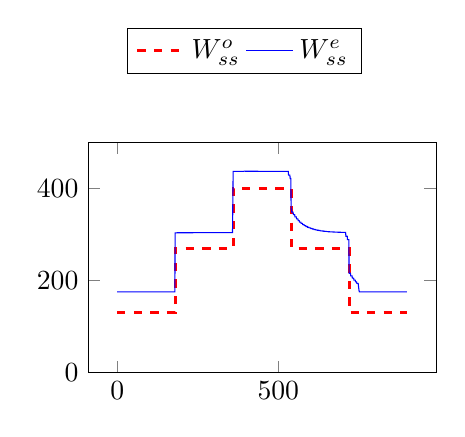
\begin{tikzpicture}
 \begin{axis}[
        height=4.5cm,
        width=6cm,
        legend style={at={(0.45,1.5)},
        anchor=north,legend columns=-1},        
        ymax=500,
        ymin=0,
  %legend cell align=left, 
        ylabel near ticks,
  ]%[name path=A]
  \addplot [red,dashed,line width=1pt] coordinates {
     (0,130) (180,130) (180,270) (360,270) (360,400) (540,400) (540,270) (720,270) (720,130) (900,130)  
  };  
  \addplot [blue] coordinates {
     (0,175) (179,175) (180,303.58984375) (181,303.58984375) (182,303.58984375) (183,303.58984375) (184,303.58984375) (185,303.58984375) (186,303.90234375) (187,303.90234375) (188,303.90234375) (189,303.90234375) (190,303.90234375) (191,303.90625) (192,303.90625) (193,303.90625) (194,303.90625) (195,303.90625) (196,303.90625) (197,303.90625) (198,303.90625) (199,303.90625) (200,303.90625) (201,303.90625) (202,303.90625) (203,303.90625) (204,303.90625) (205,303.90625) (206,303.90625) (207,303.90625) (208,303.90625) (209,303.90625) (210,303.90625) (211,303.90625) (212,303.90625) (213,303.90625) (214,303.90625) (215,303.90625) (216,303.90625) (217,303.90625) (218,303.90625) (219,303.90625) (220,303.90625) (221,303.90625) (222,303.90625) (223,303.90625) (224,303.90625) (225,303.90625) (226,303.90625) (227,303.90625) (228,303.90625) (229,303.90625) (230,303.90625) (231,303.90625) (232,303.90625) (233,303.90625) (234,303.90625) (235,303.90625) (236,303.9140625) (237,303.9140625) (238,303.9140625) (239,303.9140625) (240,303.9140625) (241,303.9140625) (242,303.9140625) (243,303.9140625) (244,303.9140625) (245,303.9140625) (246,303.9140625) (247,303.9140625) (248,303.9140625) (249,303.9140625) (250,303.9140625) (251,303.9140625) (252,303.9140625) (253,303.9140625) (254,303.9140625) (255,303.9140625) (256,303.9140625) (257,303.9140625) (258,303.9140625) (259,303.9140625) (260,303.9140625) (261,303.9140625) (262,303.9140625) (263,303.9140625) (264,303.9140625) (265,303.9140625) (266,303.9140625) (267,303.9140625) (268,303.9140625) (269,303.9140625) (270,303.9140625) (271,303.9140625) (272,303.9140625) (273,303.9140625) (274,303.9140625) (275,303.9140625) (276,303.9140625) (277,303.9140625) (278,303.9140625) (279,303.9140625) (280,303.9140625) (281,303.9140625) (282,303.9140625) (283,303.9140625) (284,303.9140625) (285,303.9140625) (286,303.9140625) (287,303.9140625) (288,303.9140625) (289,303.9140625) (290,303.9140625) (291,303.9140625) (292,303.9140625) (293,303.9140625) (294,303.9140625) (295,303.9140625) (296,303.9140625) (297,303.9140625) (298,303.9140625) (299,303.9140625) (300,303.9140625) (301,303.9140625) (302,303.9140625) (303,303.9140625) (304,303.9140625) (305,303.9140625) (306,303.9140625) (307,303.9140625) (308,303.9140625) (309,303.9140625) (310,303.9140625) (311,303.9140625) (312,303.9140625) (313,303.9140625) (314,303.9140625) (315,303.9140625) (316,303.9140625) (317,303.9140625) (318,303.9140625) (319,303.9140625) (320,303.91796875) (321,303.91796875) (322,303.91796875) (323,303.91796875) (324,303.91796875) (325,303.91796875) (326,303.91796875) (327,303.91796875) (328,303.91796875) (329,303.91796875) (330,303.91796875) (331,303.91796875) (332,303.91796875) (333,303.91796875) (334,303.91796875) (335,303.91796875) (336,303.91796875) (337,303.91796875) (338,303.91796875) (339,303.91796875) (340,303.91796875) (341,303.91796875) (342,303.91796875) (343,303.91796875) (344,303.91796875) (345,304.06640625) (346,304.06640625) (347,304.06640625) (348,304.06640625) (349,304.05078125) (350,304.05078125) (351,304.05078125) (352,304.05078125) (353,304.05078125) (354,304.03515625) (355,304.03515625) (356,304.03515625) (357,304.03515625) (358,304.03515625) (359,370.69140625) (360,437.359375) (361,437.359375) (362,437.359375) (363,437.359375) (364,437.3671875) (365,437.3671875) (366,437.3671875) (367,437.3671875) (368,437.3671875) (369,437.3671875) (370,437.3671875) (371,437.3671875) (372,437.3671875) (373,437.3671875) (374,437.3671875) (375,437.3671875) (376,437.3671875) (377,437.3671875) (378,437.3671875) (379,437.3671875) (380,437.3671875) (381,437.3671875) (382,437.3671875) (383,437.3671875) (384,437.3671875) (385,437.3671875) (386,437.3671875) (387,437.3671875) (388,437.3671875) (389,437.3671875) (390,437.3671875) (391,437.3671875) (392,437.3671875) (393,437.3671875) (394,437.7265625) (395,437.7265625) (396,437.7265625) (397,437.7265625) (398,437.68359375) (399,437.68359375) (400,437.68359375) (401,437.68359375) (402,437.68359375) (403,437.64453125) (404,437.64453125) (405,437.64453125) (406,437.64453125) (407,437.64453125) (408,437.61328125) (409,437.61328125) (410,437.61328125) (411,437.61328125) (412,437.61328125) (413,437.5859375) (414,437.5859375) (415,437.5859375) (416,437.5859375) (417,437.5859375) (418,437.55859375) (419,437.55859375) (420,437.55859375) (421,437.55859375) (422,437.55859375) (423,437.53515625) (424,437.53515625) (425,437.53515625) (426,437.53515625) (427,437.53515625) (428,437.515625) (429,437.515625) (430,437.515625) (431,437.515625) (432,437.515625) (433,437.5) (434,437.5) (435,437.5) (436,437.5) (437,437.5) (438,437.484375) (439,437.484375) (440,437.484375) (441,437.484375) (442,437.484375) (443,437.47265625) (444,437.47265625) (445,437.47265625) (446,437.47265625) (447,437.47265625) (448,437.4609375) (449,437.4609375) (450,437.4609375) (451,437.4609375) (452,437.4609375) (453,437.453125) (454,437.453125) (455,437.453125) (456,437.453125) (457,437.453125) (458,437.4453125) (459,437.4453125) (460,437.4453125) (461,437.4453125) (462,437.4453125) (463,437.4375) (464,437.4375) (465,437.4375) (466,437.4375) (467,437.4375) (468,437.4296875) (469,437.4296875) (470,437.4296875) (471,437.4296875) (472,437.4296875) (473,437.42578125) (474,437.42578125) (475,437.42578125) (476,437.42578125) (477,437.421875) (478,437.421875) (479,437.421875) (480,437.421875) (481,437.421875) (482,437.41796875) (483,437.41796875) (484,437.41796875) (485,437.41796875) (486,437.41796875) (487,437.4140625) (488,437.4140625) (489,437.4140625) (490,437.4140625) (491,437.4140625) (492,437.41015625) (493,437.41015625) (494,437.41015625) (495,437.41015625) (496,437.41015625) (497,437.40625) (498,437.40625) (499,437.40625) (500,437.40625) (501,437.40625) (502,437.40625) (503,437.40625) (504,437.40625) (505,437.40625) (506,437.40625) (507,437.40625) (508,437.40625) (509,437.40625) (510,437.40625) (511,437.40625) (512,437.40625) (513,437.40625) (514,437.40625) (515,437.40625) (516,437.40625) (517,437.40625) (518,437.40625) (519,437.40625) (520,437.40625) (521,437.40625) (522,437.40625) (523,437.40625) (524,437.40625) (525,437.40625) (526,437.40625) (527,437.40625) (528,437.40625) (529,437.40625) (530,437.40625) (531,437.40625) (532,429.0625) (533,429.0625) (534,429.0625) (535,429.0625) (536,429.0625) (537,421.76171875) (538,421.76171875) (539,421.76171875) (540,355.09375) (541,355.09375) (542,348.703125) (543,348.703125) (544,348.703125) (545,348.703125) (546,348.703125) (547,343.11328125) (548,343.11328125) (549,343.11328125) (550,343.11328125) (551,343.11328125) (552,338.22265625) (553,338.22265625) (554,338.22265625) (555,338.22265625) (556,338.22265625) (557,333.94140625) (558,333.94140625) (559,333.94140625) (560,333.94140625) (561,333.94140625) (562,330.1953125) (563,330.1953125) (564,330.1953125) (565,330.1953125) (566,326.91796875) (567,326.91796875) (568,326.91796875) (569,326.91796875) (570,326.91796875) (571,324.05078125) (572,324.05078125) (573,324.05078125) (574,324.05078125) (575,324.05078125) (576,321.54296875) (577,321.54296875) (578,321.54296875) (579,321.54296875) (580,321.54296875) (581,319.34765625) (582,319.34765625) (583,319.34765625) (584,319.34765625) (585,319.34765625) (586,317.42578125) (587,317.42578125) (588,317.42578125) (589,317.42578125) (590,317.42578125) (591,315.74609375) (592,315.74609375) (593,315.74609375) (594,315.74609375) (595,315.74609375) (596,314.27734375) (597,314.27734375) (598,314.27734375) (599,314.27734375) (600,314.27734375) (601,312.9921875) (602,312.9921875) (603,312.9921875) (604,312.9921875) (605,312.9921875) (606,311.8671875) (607,311.8671875) (608,311.8671875) (609,311.8671875) (610,311.8671875) (611,310.8828125) (612,310.8828125) (613,310.8828125) (614,310.8828125) (615,310.8828125) (616,310.01953125) (617,310.01953125) (618,310.01953125) (619,310.01953125) (620,310.01953125) (621,309.265625) (622,309.265625) (623,309.265625) (624,309.265625) (625,309.265625) (626,308.60546875) (627,308.60546875) (628,308.60546875) (629,308.60546875) (630,308.60546875) (631,308.02734375) (632,308.02734375) (633,308.02734375) (634,308.02734375) (635,308.02734375) (636,307.5234375) (637,307.5234375) (638,307.5234375) (639,307.5234375) (640,307.5234375) (641,307.08203125) (642,307.08203125) (643,307.08203125) (644,307.08203125) (645,307.08203125) (646,306.6953125) (647,306.6953125) (648,306.6953125) (649,306.6953125) (650,306.6953125) (651,306.359375) (652,306.359375) (653,306.359375) (654,306.359375) (655,306.0625) (656,306.0625) (657,306.0625) (658,306.0625) (659,306.0625) (660,305.8046875) (661,305.8046875) (662,305.8046875) (663,305.8046875) (664,305.8046875) (665,305.578125) (666,305.578125) (667,305.578125) (668,305.578125) (669,305.578125) (670,305.37890625) (671,305.37890625) (672,305.37890625) (673,305.37890625) (674,305.37890625) (675,305.20703125) (676,305.20703125) (677,305.20703125) (678,305.20703125) (679,305.20703125) (680,305.0546875) (681,305.0546875) (682,305.0546875) (683,305.0546875) (684,305.0546875) (685,304.921875) (686,304.921875) (687,304.921875) (688,304.921875) (689,304.921875) (690,304.8046875) (691,304.8046875) (692,304.8046875) (693,304.8046875) (694,304.8046875) (695,304.703125) (696,304.703125) (697,304.703125) (698,304.703125) (699,304.703125) (700,304.61328125) (701,304.61328125) (702,304.61328125) (703,304.61328125) (704,304.61328125) (705,304.53515625) (706,304.53515625) (707,304.53515625) (708,304.53515625) (709,304.53515625) (710,296.1171875) (711,296.1171875) (712,296.1171875) (713,296.1171875) (714,296.1171875) (715,288.75390625) (716,288.75390625) (717,288.75390625) (718,288.75390625) (719,288.75390625) (720,215.642578125) (721,215.642578125) (722,215.642578125) (723,215.642578125) (724,215.642578125) (725,210.005859375) (726,210.005859375) (727,210.005859375) (728,210.005859375) (729,210.005859375) (730,205.068359375) (731,205.068359375) (732,205.068359375) (733,205.068359375) (734,205.068359375) (735,200.751953125) (736,200.751953125) (737,200.751953125) (738,200.751953125) (739,200.751953125) (740,196.974609375) (741,196.974609375) (742,196.974609375) (743,196.974609375) (744,193.669921875) (745,193.669921875) (746,193.669921875) (747,193.669921875) (748,193.669921875) (749,187.853515625) (750,182.2236328125) (751,176.7568359375) (752,175) (899,175)
  };       
  \legend{$W^o_{ss}$,$W^{e}_{ss}$}  
 \end{axis}
\end{tikzpicture}
   
 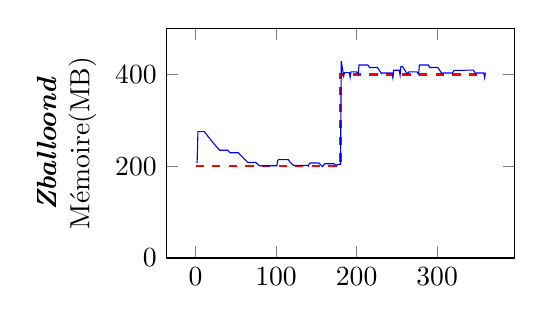
\begin{tikzpicture}
 \begin{axis}[
        height=4.5cm,
        width=6cm,
        %legend style={at={(0.5,1.3)}, anchor=north,legend columns=-1},        
        ymax=500,
        ymin=0,
  %legend cell align=left, 
        ylabel near ticks,
        ylabel style={align=center},
        ylabel={\textbf{{\em Zballoond}}\\Mémoire(MB)},
  ]%[name path=A]
   \addplot [red,dashed,line width=1pt] coordinates {  
    (0,200) (180,200) (180,400) (360,400)
   };   
   \addplot [blue] coordinates {
    (1,208.390625) (2,208.390625) (3,275.1015625) (4,275.1015625) (5,275.1015625) (6,275.1015625) (7,275.1015625) (8,275.1015625) (9,275.1015625) (10,275.1015625) (11,275.1015625) (12,272.765625) (13,270.453125) (14,268.1640625) (15,265.8984375) (16,263.65625) (17,261.4375) (18,259.23828125) (19,257.0625) (20,254.90625) (21,252.7734375) (22,250.66015625) (23,248.5703125) (24,246.5) (25,244.44921875) (26,242.421875) (27,240.4140625) (28,238.42578125) (29,236.45703125) (30,234.5078125) (31,234.515625) (32,234.515625) (33,234.515625) (34,234.515625) (35,234.515625) (36,234.515625) (37,234.515625) (38,234.515625) (39,234.515625) (40,234.515625) (41,232.5859375) (42,230.67578125) (43,228.78515625) (44,229.16015625) (45,229.16015625) (46,229.16015625) (47,229.16015625) (48,229.16015625) (49,229.16015625) (50,229.16015625) (51,229.16015625) (52,229.16015625) (53,229.16015625) (54,227.28515625) (55,225.4296875) (56,223.58984375) (57,221.76953125) (58,219.96875) (59,218.18359375) (60,216.41796875) (61,214.66796875) (62,212.9375) (63,211.22265625) (64,209.52734375) (65,207.84765625) (66,207.85546875) (67,207.85546875) (68,207.85546875) (69,207.85546875) (70,207.85546875) (71,207.85546875) (72,207.85546875) (73,207.85546875) (74,207.85546875) (75,207.85546875) (76,206.19140625) (77,204.546875) (78,202.91796875) (79,201.3046875) (80,200.49609375) (81,200.84765625) (82,200.84765625) (83,200.84765625) (84,200.84765625) (85,200.84765625) (86,200.84765625) (87,200.84765625) (88,200.84765625) (89,200.84765625) (90,200.84765625) (91,199.25390625) (92,200.55859375) (93,200.6640625) (94,200.6640625) (95,200.6640625) (96,200.70703125) (97,200.70703125) (98,200.70703125) (99,200.70703125) (100,200.70703125) (101,200.70703125) (102,212.33203125) (103,214.21875) (104,214.21875) (105,214.21875) (106,214.25390625) (107,214.25390625) (108,214.25390625) (109,214.25390625) (110,214.25390625) (111,214.25390625) (112,214.25390625) (113,214.25390625) (114,214.25390625) (115,214.25390625) (116,212.52734375) (117,209.125) (118,207.44921875) (119,205.7890625) (120,204.1484375) (121,202.5234375) (122,200.9140625) (123,201.5234375) (124,201.5234375) (125,201.5234375) (126,201.5234375) (127,201.5234375) (128,201.5234375) (129,201.5234375) (130,201.5546875) (131,201.5546875) (132,201.5546875) (133,201.5546875) (134,201.5546875) (135,201.5546875) (136,201.5546875) (137,201.5546875) (138,201.5546875) (139,201.5546875) (140,199.95703125) (141,204.18359375) (142,206.77734375) (143,206.77734375) (144,206.8125) (145,206.8125) (146,206.8125) (147,206.8125) (148,206.8125) (149,206.8125) (150,206.8125) (151,206.8125) (152,206.8125) (153,206.8125) (154,205.16015625) (155,203.5234375) (156,201.90234375) (157,200.30078125) (158,198.71484375) (159,202.28125) (160,204.34765625) (161,205.17578125) (162,205.17578125) (163,205.17578125) (164,205.2109375) (165,205.2109375) (166,205.2109375) (167,205.2109375) (168,205.2109375) (169,205.2109375) (170,205.2109375) (171,205.2109375) (172,205.2109375) (173,203.57421875) (174,201.953125) (175,200.34765625) (176,203.57421875) (177,203.57421875) (178,203.57421875) (179,203.57421875) (180,203.57421875) (181,428.359375) (182,416.94140625) (183,406.09375) (184,395.7890625) (185,403.333984375) (186,403.333984375) (187,403.333984375) (188,403.333984375) (189,403.333984375) (190,403.333984375) (191,403.333984375) (192,393.1669921875) (193,405.09765625) (194,405.09765625) (195,405.09765625) (196,405.09765625) (197,405.09765625) (198,405.09765625) (199,405.09765625) (200,405.09765625) (201,402.4609375) (202,399.8515625) (203,419.90234375) (204,419.9375) (205,420.01171875) (206,420.01171875) (207,420.01171875) (208,420.01171875) (209,420.01171875) (210,420.01171875) (211,420.01171875) (212,420.01171875) (213,420.01171875) (214,420.01171875) (215,417.2265625) (216,414.46875) (217,414.4765625) (218,414.4765625) (219,414.4765625) (220,414.4765625) (221,414.4765625) (222,414.4765625) (223,414.4765625) (224,414.4765625) (225,414.4765625) (226,414.4765625) (227,411.74609375) (228,409.04296875) (229,406.3671875) (230,403.71875) (231,401.09765625) (232,402.49609375) (233,402.49609375) (234,402.49609375) (235,402.53125) (236,402.53125) (237,402.53125) (238,402.53125) (239,402.53125) (240,402.53125) (241,402.53125) (242,402.53125) (243,402.53125) (244,402.53125) (245,392.44140625) (246,408.52734375) (247,408.52734375) (248,408.52734375) (249,408.52734375) (250,408.52734375) (251,408.52734375) (252,408.52734375) (253,408.52734375) (254,398.1005859375) (255,416.6953125) (256,416.6953125) (257,416.6953125) (258,413.9453125) (259,411.22265625) (260,408.52734375) (261,405.859375) (262,403.21484375) (263,400.59765625) (264,403.18359375) (265,405.0625) (266,405.09765625) (267,405.09765625) (268,405.09765625) (269,405.09765625) (270,405.09765625) (271,405.09765625) (272,405.09765625) (273,405.09765625) (274,405.09765625) (275,405.09765625) (276,402.4609375) (277,399.8515625) (278,419.90234375) (279,419.9375) (280,420.01171875) (281,420.01171875) (282,420.01171875) (283,420.01171875) (284,420.01171875) (285,420.01171875) (286,420.01171875) (287,420.01171875) (288,420.01171875) (289,420.01171875) (290,417.2265625) (291,414.46875) (292,414.4765625) (293,414.4765625) (294,414.4765625) (295,414.4765625) (296,414.4765625) (297,414.4765625) (298,414.4765625) (299,414.4765625) (300,414.4765625) (301,414.4765625) (302,411.74609375) (303,409.04296875) (304,406.3671875) (305,403.71875) (306,401.09765625) (307,402.49609375) (308,402.49609375) (309,402.49609375) (310,402.53125) (311,402.53125) (312,402.53125) (313,402.53125) (314,402.53125) (315,402.53125) (316,402.53125) (317,402.53125) (318,402.53125) (319,402.53125) (320,405.4453125) (321,408.3203125) (322,408.3203125) (323,408.3203125) (324,408.35546875) (325,408.35546875) (326,408.36328125) (327,408.36328125) (328,408.36328125) (329,408.36328125) (330,408.36328125) (331,408.36328125) (332,408.36328125) (333,408.36328125) (334,408.36328125) (335,408.36328125) (336,408.85546875) (337,408.85546875) (338,408.85546875) (339,408.85546875) (340,408.85546875) (341,408.85546875) (342,408.85546875) (343,408.85546875) (344,408.85546875) (345,408.85546875) (346,406.18359375) (347,403.5390625) (348,400.91796875) (349,402.52734375) (350,402.52734375) (351,402.52734375) (352,402.52734375) (353,402.52734375) (354,402.52734375) (355,402.52734375) (356,402.52734375) (357,402.52734375) (358,402.52734375) (359,392.400390625) (360,403.27734375)
  }; 
  %\legend{$W^o_{3}$,$W^{e}_{3,d}$}        
\end{axis}  
\end{tikzpicture}
%%%%%%%%%%%%%%%%%%%%%%%%%%%%%%%%%%%%%%%%%%%%%%%%%%%%%
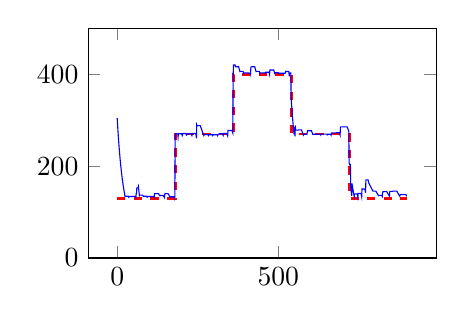
\begin{tikzpicture}
 \begin{axis}[
        height=4.5cm,
        width=6cm,
        %legend style={at={(0.5,1.3)}, anchor=north,legend columns=-1},        
        ymax=500,
        ymin=0,
  %legend cell align=left, 
        ylabel near ticks,
  ]%[name path=A]
    \addplot [red,dashed,line width=1pt] coordinates {  
         (0,130) (180,130) (180,270) (360,270) (360,400) (540,400) (540,270) (720,270) (720,130) (900,130)
    };    
  \addplot [blue] coordinates {
    (0,304.349609375) (1,292.46484375) (2,281.1748046875) (3,270.44921875) (4,260.2607421875) (5,250.580078125) (6,241.384765625) (7,232.6484375) (8,224.349609375) (9,216.4658203125) (10,208.9755859375) (11,201.8603515625) (12,195.1005859375) (13,188.6787109375) (14,182.578125) (15,176.7822265625) (16,171.2763671875) (17,166.0458984375) (18,161.0771484375) (19,156.3564453125) (20,151.8720703125) (21,147.611328125) (22,143.564453125) (23,139.71875) (24,134.501953125) (25,134.505859375) (26,134.505859375) (27,134.505859375) (28,134.505859375) (29,134.505859375) (30,134.505859375) (31,134.505859375) (32,134.505859375) (33,134.505859375) (34,134.505859375) (35,133.341796875) (36,132.189453125) (37,133.876953125) (38,133.912109375) (39,133.912109375) (40,133.912109375) (41,133.912109375) (42,133.919921875) (43,133.919921875) (44,133.919921875) (45,133.919921875) (46,133.919921875) (47,133.935546875) (48,133.935546875) (49,133.935546875) (50,133.935546875) (51,133.935546875) (52,133.935546875) (53,133.935546875) (54,133.935546875) (55,133.935546875) (56,133.935546875) (57,132.775390625) (58,131.626953125) (59,140.244140625) (60,140.244140625) (61,152.513671875) (62,152.529296875) (63,152.537109375) (64,152.537109375) (65,152.537109375) (66,155.373046875) (67,148.498046875) (68,141.966796875) (69,135.763671875) (70,136.787109375) (71,136.787109375) (72,136.787109375) (73,136.787109375) (74,136.787109375) (75,136.787109375) (76,136.787109375) (77,136.787109375) (78,136.787109375) (79,136.787109375) (80,135.599609375) (81,134.501953125) (82,134.505859375) (83,134.505859375) (84,134.505859375) (85,134.505859375) (86,134.505859375) (87,134.505859375) (88,134.505859375) (89,134.505859375) (90,134.505859375) (91,134.505859375) (92,133.341796875) (93,132.189453125) (94,133.876953125) (95,133.912109375) (96,133.912109375) (97,133.912109375) (98,133.912109375) (99,133.919921875) (100,133.919921875) (101,133.919921875) (102,133.919921875) (103,133.919921875) (104,133.935546875) (105,133.935546875) (106,133.935546875) (107,133.935546875) (108,133.935546875) (109,133.935546875) (110,133.935546875) (111,133.935546875) (112,133.935546875) (113,133.935546875) (114,132.775390625) (115,131.626953125) (116,140.244140625) (117,140.244140625) (118,140.244140625) (119,140.279296875) (120,140.279296875) (121,140.279296875) (122,140.279296875) (123,140.279296875) (124,140.279296875) (125,140.279296875) (126,140.279296875) (127,140.279296875) (128,140.279296875) (129,139.056640625) (130,137.845703125) (131,136.646484375) (132,135.458984375) (133,135.462890625) (134,136.056640625) (135,136.056640625) (136,136.056640625) (137,136.056640625) (138,136.056640625) (139,136.056640625) (140,136.056640625) (141,136.056640625) (142,136.056640625) (143,136.056640625) (144,134.876953125) (145,133.708984375) (146,132.552734375) (147,131.408203125) (148,140.013671875) (149,140.017578125) (150,140.017578125) (151,140.017578125) (152,140.017578125) (153,140.017578125) (154,140.017578125) (155,140.017578125) (156,140.017578125) (157,140.017578125) (158,140.017578125) (159,138.798828125) (160,137.591796875) (161,136.396484375) (162,135.212890625) (163,134.041015625) (164,132.880859375) (165,131.732421875) (166,133.208984375) (167,133.216796875) (168,133.216796875) (169,133.216796875) (170,133.216796875) (171,133.216796875) (172,133.216796875) (173,133.216796875) (174,133.216796875) (175,133.216796875) (176,133.216796875) (177,129.888671875) (178,133.4140625) (179,133.4140625) (180,258.453125) (181,270.1181640625) (182,270.1181640625) (183,270.1181640625) (184,270.1181640625) (185,270.1181640625) (186,270.1181640625) (187,270.1181640625) (188,270.1181640625) (189,263.2783203125) (190,270.32421875) (191,270.32421875) (192,270.33203125) (193,270.33203125) (194,270.33203125) (195,270.33203125) (196,270.33203125) (197,270.33203125) (198,270.33203125) (199,270.33203125) (200,270.33203125) (201,268.4765625) (202,266.640625) (203,269.34765625) (204,270.99609375) (205,270.99609375) (206,270.99609375) (207,270.99609375) (208,270.99609375) (209,270.99609375) (210,270.99609375) (211,270.99609375) (212,270.99609375) (213,270.99609375) (214,269.1328125) (215,267.2890625) (216,268.07421875) (217,269.64453125) (218,269.64453125) (219,269.64453125) (220,270.32421875) (221,270.32421875) (222,270.33203125) (223,270.33203125) (224,270.33203125) (225,270.33203125) (226,270.33203125) (227,270.33203125) (228,270.33203125) (229,270.33203125) (230,270.33203125) (231,268.4765625) (232,266.640625) (233,269.34765625) (234,270.99609375) (235,270.99609375) (236,270.99609375) (237,270.99609375) (238,270.99609375) (239,270.99609375) (240,270.99609375) (241,270.99609375) (242,270.99609375) (243,270.99609375) (244,269.1328125) (245,267.2890625) (246,260.5908203125) (247,289.96875) (248,287.91796875) (249,287.92578125) (250,287.92578125) (251,287.92578125) (252,287.92578125) (253,287.92578125) (254,287.92578125) (255,287.92578125) (256,287.92578125) (257,287.92578125) (258,287.92578125) (259,285.89453125) (260,283.8828125) (261,281.890625) (262,279.91796875) (263,277.96484375) (264,276.03125) (265,274.1171875) (266,272.22265625) (267,270.34765625) (268,268.4921875) (269,266.65234375) (270,268.3984375) (271,268.3984375) (272,268.3984375) (273,268.4296875) (274,268.4296875) (275,268.4296875) (276,268.4296875) (277,268.4296875) (278,268.4296875) (279,268.4296875) (280,268.4296875) (281,268.4296875) (282,268.4296875) (283,266.59375) (284,268.28515625) (285,268.28515625) (286,268.28515625) (287,268.296875) (288,268.296875) (289,268.296875) (290,268.296875) (291,268.296875) (292,268.296875) (293,268.296875) (294,268.296875) (295,268.296875) (296,268.296875) (297,266.4609375) (298,268.12109375) (299,268.12109375) (300,268.12109375) (301,268.12109375) (302,268.1484375) (303,268.1484375) (304,268.1484375) (305,268.1484375) (306,268.1484375) (307,268.1484375) (308,268.1484375) (309,268.1484375) (310,268.1484375) (311,268.1484375) (312,266.3125) (313,268.07421875) (314,269.64453125) (315,269.64453125) (316,269.64453125) (317,270.32421875) (318,270.32421875) (319,270.33203125) (320,270.33203125) (321,270.33203125) (322,270.33203125) (323,270.33203125) (324,270.33203125) (325,270.33203125) (326,270.33203125) (327,270.33203125) (328,268.4765625) (329,266.640625) (330,269.34765625) (331,270.99609375) (332,270.99609375) (333,270.99609375) (334,270.99609375) (335,270.99609375) (336,270.99609375) (337,270.99609375) (338,270.99609375) (339,270.99609375) (340,270.99609375) (341,269.1328125) (342,267.2890625) (343,265.46484375) (344,277.54296875) (345,277.54296875) (346,277.578125) (347,277.5859375) (348,277.5859375) (349,277.5859375) (350,277.5859375) (351,277.5859375) (352,277.5859375) (353,277.5859375) (354,277.5859375) (355,277.5859375) (356,277.5859375) (357,275.65625) (358,273.74609375) (359,271.85546875) (360,393.568359375) (361,420.408203125) (362,420.408203125) (363,420.408203125) (364,420.408203125) (365,420.408203125) (366,420.408203125) (367,416.05078125) (368,416.0859375) (369,416.0859375) (370,416.0859375) (371,416.0859375) (372,416.0859375) (373,416.0859375) (374,416.0859375) (375,416.0859375) (376,416.0859375) (377,416.0859375) (378,413.4375) (379,410.81640625) (380,408.22265625) (381,405.65234375) (382,406.03515625) (383,406.03515625) (384,406.03515625) (385,406.03515625) (386,406.03515625) (387,406.03515625) (388,406.03515625) (389,406.03515625) (390,406.03515625) (391,406.03515625) (392,403.48828125) (393,400.96875) (394,402.6796875) (395,402.6796875) (396,402.6796875) (397,402.6796875) (398,402.71484375) (399,402.72265625) (400,402.72265625) (401,402.72265625) (402,402.72265625) (403,402.72265625) (404,402.72265625) (405,402.72265625) (406,402.72265625) (407,402.72265625) (408,402.72265625) (409,401.66015625) (410,401.66015625) (411,401.66015625) (412,401.66015625) (413,402.70703125) (414,400.1953125) (415,415.3125) (416,416.05078125) (417,416.05078125) (418,416.0859375) (419,416.0859375) (420,416.0859375) (421,416.0859375) (422,416.0859375) (423,416.0859375) (424,416.0859375) (425,416.0859375) (426,416.0859375) (427,416.0859375) (428,413.4375) (429,410.81640625) (430,408.22265625) (431,405.65234375) (432,406.03515625) (433,406.03515625) (434,406.03515625) (435,406.03515625) (436,406.03515625) (437,406.03515625) (438,406.03515625) (439,406.03515625) (440,406.03515625) (441,406.03515625) (442,403.48828125) (443,400.96875) (444,402.6796875) (445,402.6796875) (446,402.6796875) (447,402.6796875) (448,402.71484375) (449,402.72265625) (450,402.72265625) (451,402.72265625) (452,402.72265625) (453,402.72265625) (454,402.72265625) (455,402.72265625) (456,402.72265625) (457,402.72265625) (458,402.72265625) (459,401.66015625) (460,404.2265625) (461,404.2265625) (462,404.26171875) (463,404.26171875) (464,404.26171875) (465,404.26171875) (466,404.26171875) (467,404.26171875) (468,404.26171875) (469,404.26171875) (470,404.26171875) (471,404.26171875) (472,401.734375) (473,399.23046875) (474,409.03125) (475,409.03125) (476,409.10546875) (477,409.11328125) (478,409.11328125) (479,409.11328125) (480,409.11328125) (481,409.11328125) (482,409.11328125) (483,409.11328125) (484,409.11328125) (485,409.11328125) (486,409.11328125) (487,406.53515625) (488,403.984375) (489,401.45703125) (490,402.140625) (491,403.265625) (492,403.265625) (493,403.265625) (494,403.265625) (495,403.265625) (496,403.265625) (497,403.265625) (498,403.265625) (499,403.265625) (500,403.265625) (501,400.74609375) (502,400.80078125) (503,401.984375) (504,401.984375) (505,401.984375) (506,402.01953125) (507,402.01953125) (508,402.01953125) (509,402.01953125) (510,402.01953125) (511,402.01953125) (512,402.02734375) (513,402.02734375) (514,402.02734375) (515,402.02734375) (516,402.02734375) (517,402.02734375) (518,402.02734375) (519,402.02734375) (520,402.02734375) (521,402.02734375) (522,403.015625) (523,405.82421875) (524,405.82421875) (525,405.859375) (526,405.859375) (527,405.859375) (528,405.859375) (529,405.859375) (530,405.859375) (531,405.859375) (532,405.859375) (533,405.859375) (534,395.56640625) (535,402.765625) (536,402.765625) (537,402.765625) (538,402.765625) (539,402.765625) (540,348.703125) (541,337.9345703125) (542,327.7041015625) (543,317.9853515625) (544,308.7529296875) (545,299.9814453125) (546,291.6494140625) (547,283.7333984375) (548,276.212890625) (549,269.0693359375) (550,284.47265625) (551,274.4765625) (552,264.98046875) (553,288.46875) (554,278.2734375) (555,278.3515625) (556,278.3515625) (557,278.3515625) (558,278.3515625) (559,278.3515625) (560,278.3515625) (561,278.3515625) (562,278.3515625) (563,278.85546875) (564,278.85546875) (565,278.85546875) (566,278.85546875) (567,278.85546875) (568,278.85546875) (569,278.85546875) (570,278.85546875) (571,278.85546875) (572,278.85546875) (573,276.9140625) (574,274.9921875) (575,273.08984375) (576,271.20703125) (577,269.34375) (578,267.49609375) (579,268.921875) (580,268.9375) (581,268.9375) (582,268.9375) (583,268.9375) (584,268.9375) (585,268.9375) (586,268.9375) (587,268.9375) (588,268.9375) (589,268.9375) (590,273.48828125) (591,276.953125
) (592,276.953125) (593,276.953125) (594,276.98828125) (595,276.98828125) (596,276.98828125) (597,276.98828125) (598,276.98828125) (599,276.98828125) (600,276.98828125) (601,276.98828125) (602,276.98828125) (603,276.98828125) (604,275.06640625) (605,273.1640625) (606,271.28125) (607,269.4140625) (608,269.421875) (609,269.421875) (610,269.421875) (611,269.421875) (612,269.421875) (613,269.42578125) (614,269.42578125) (615,269.42578125) (616,269.42578125) (617,269.42578125) (618,269.42578125) (619,269.42578125) (620,269.42578125) (621,269.42578125) (622,269.734375) (623,269.734375) (624,269.734375) (625,269.734375) (626,269.734375) (627,269.734375) (628,269.734375) (629,269.734375) (630,269.734375) (631,269.734375) (632,267.8828125) (633,269.67578125) (634,269.67578125) (635,269.67578125) (636,269.67578125) (637,269.67578125) (638,269.67578125) (639,269.67578125) (640,269.67578125) (641,269.67578125) (642,269.68359375) (643,269.68359375) (644,269.68359375) (645,269.68359375) (646,269.68359375) (647,269.68359375) (648,269.68359375) (649,269.68359375) (650,269.68359375) (651,269.68359375) (652,267.83203125) (653,268.125) (654,269.26171875) (655,269.26171875) (656,269.26171875) (657,269.26171875) (658,269.26171875) (659,269.26171875) (660,269.26171875) (661,269.26171875) (662,269.26171875) (663,269.26171875) (664,267.41796875) (665,270.2890625) (666,272.140625) (667,272.140625) (668,272.20703125) (669,272.20703125) (670,272.20703125) (671,272.20703125) (672,272.20703125) (673,272.20703125) (674,272.20703125) (675,272.20703125) (676,272.20703125) (677,272.21484375) (678,272.21484375) (679,272.21484375) (680,272.21484375) (681,272.88671875) (682,272.88671875) (683,272.88671875) (684,272.88671875) (685,272.88671875) (686,272.88671875) (687,272.88671875) (688,272.88671875) (689,272.88671875) (690,271.00390625) (691,269.140625) (692,267.296875) (693,284.85546875) (694,285.43359375) (695,285.43359375) (696,285.46875) (697,285.46875) (698,285.46875) (699,285.46875) (700,285.46875) (701,285.46875) (702,285.46875) (703,285.46875) (704,285.46875) (705,285.4765625) (706,285.4765625) (707,285.4765625) (708,285.4765625) (709,285.4765625) (710,285.4765625) (711,285.4765625) (712,285.4765625) (713,285.4765625) (714,285.4765625) (715,283.46875) (716,281.48046875) (717,279.51171875) (718,277.5625) (719,275.6328125) (720,207.056640625) (721,205.166015625) (722,203.294921875) (723,201.443359375) (724,202.302734375) (725,155.169921875) (726,148.306640625) (727,141.783203125) (728,135.587890625) (729,162.287109375) (730,157.505859375) (731,152.9638671875) (732,148.6484375) (733,144.5498046875) (734,140.6552734375) (735,136.9560546875) (736,133.44140625) (737,139.48046875) (738,139.48046875) (739,139.48046875) (740,139.48046875) (741,139.48046875) (742,139.48046875) (743,139.48046875) (744,139.48046875) (745,139.48046875) (746,135.8876953125) (747,132.42578125) (748,140.525390625) (749,140.525390625) (750,140.525390625) (751,140.525390625) (752,140.525390625) (753,140.525390625) (754,140.525390625) (755,140.525390625) (756,140.525390625) (757,140.525390625) (758,136.83203125) (759,133.3232421875) (760,150.2802734375) (761,150.2802734375) (762,150.2802734375) (763,150.2802734375) (764,150.2802734375) (765,150.2802734375) (766,150.2802734375) (767,150.2802734375) (768,150.2802734375) (769,150.2802734375) (770,146.0986328125) (771,142.126953125) (772,169.9453125) (773,169.9453125) (774,169.9453125) (775,169.9453125) (776,169.9453125) (777,169.9453125) (778,169.9453125) (779,169.9453125) (780,164.806640625) (781,163.337890625) (782,161.884765625) (783,160.447265625) (784,159.021484375) (785,157.611328125) (786,156.216796875) (787,154.833984375) (788,153.466796875) (789,152.111328125) (790,150.771484375) (791,149.443359375) (792,148.130859375) (793,146.830078125) (794,145.541015625) (795,145.548828125) (796,145.548828125) (797,145.548828125) (798,145.548828125) (799,145.548828125) (800,145.548828125) (801,145.548828125) (802,145.548828125) (803,145.548828125) (804,144.275390625) (805,143.013671875) (806,141.763671875) (807,140.525390625) (808,139.298828125) (809,138.087890625) (810,136.888671875) (811,135.701171875) (812,136.353515625) (813,136.353515625) (814,136.353515625) (815,136.353515625) (816,136.353515625) (817,136.353515625) (818,136.353515625) (819,136.353515625) (820,136.353515625) (821,136.353515625) (822,135.169921875) (823,133.998046875) (824,143.220703125) (825,144.279296875) (826,144.279296875) (827,144.279296875) (828,144.322265625) (829,144.322265625) (830,144.322265625) (831,144.322265625) (832,144.322265625) (833,144.322265625) (834,144.322265625) (835,144.322265625) (836,144.322265625) (837,144.322265625) (838,143.060546875) (839,141.810546875) (840,140.572265625) (841,139.345703125) (842,138.130859375) (843,136.931640625) (844,135.744140625) (845,134.568359375) (846,143.873046875) (847,144.896484375) (848,144.896484375) (849,144.896484375) (850,144.896484375) (851,144.896484375) (852,144.896484375) (853,144.896484375) (854,144.896484375) (855,145.587890625) (856,145.587890625) (857,145.595703125) (858,145.595703125) (859,145.603515625) (860,145.603515625) (861,145.603515625) (862,145.603515625) (863,145.603515625) (864,145.603515625) (865,145.603515625) (866,145.603515625) (867,145.603515625) (868,145.603515625) (869,144.326171875) (870,143.064453125) (871,141.814453125) (872,140.576171875) (873,139.349609375) (874,138.134765625) (875,136.935546875) (876,135.748046875) (877,134.572265625) (878,136.564453125) (879,137.923828125) (880,137.923828125) (881,137.923828125) (882,137.958984375) (883,137.958984375) (884,137.958984375) (885,137.958984375) (886,137.958984375) (887,137.958984375) (888,137.978515625) (889,137.978515625) (890,137.978515625) (891,137.978515625) (892,137.978515625) (893,137.978515625) (894,137.978515625) (895,137.978515625) (896,137.978515625) (897,136.779296875) (898,135.591796875) (899,134.416015625)
  };  
  %\legend{$W^o_{5}$,$W^{e}_{5,d}$}      
 \end{axis}
\end{tikzpicture}

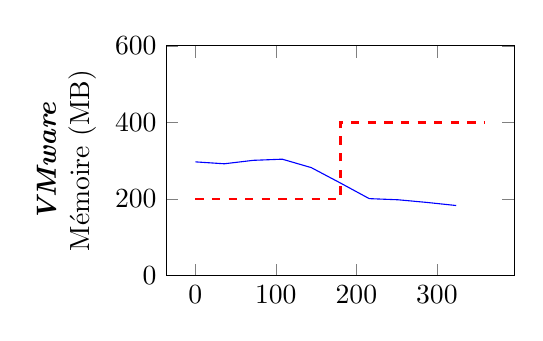
\begin{tikzpicture}
 \begin{axis}[
        height=4.5cm,
        width=6cm,
        %legend style={at={(0.5,1.45)}, anchor=north,legend columns=-1},        
        ymax=600,
        ymin=0,
  %legend cell align=left, 
        ylabel near ticks,
        ylabel style={align=center}, 
        ylabel={\textbf{{\em VMware}}\\Mémoire (MB)},
  ]%[name path=A]
  \addplot [red,dashed,line width=1pt] coordinates {
    (0,200) (180,200) (180,400) (360,400)
  };  
  \addplot [blue] coordinates {
    (0,297) (36,292) (72,301) (108,304) (144,282) (180,242) (216,201) (252,198) (288,191) (324,183)
  }; 
  %\legend{$W^o_{3}$,$W^e_{3}$}        
\end{axis}  
\end{tikzpicture} 
%%%%%%%%%%%%%%%%%%%%%%%%%%%%%%%%%%%%%%%%%%%%%%%%%%%%%
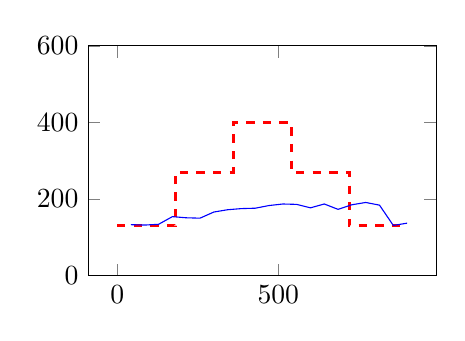
\begin{tikzpicture}
 \begin{axis}[
        height=4.5cm,
        width=6cm,
        %legend style={at={(0.5,1.45)}, anchor=north,legend columns=-1},        
        ymax=600,
        ymin=0,
  %legend cell align=left, 
        ylabel near ticks,
  ]%[name path=A]
  \addplot [red,dashed,line width=1pt] coordinates {
     (0,130) (180,130) (180,270) (360,270) (360,400) (540,400) (540,270) (720,270) (720,130) (900,130)  
  };   
  \addplot [blue] coordinates {
         (42.8571428571,133) (85.7142857143,132) (128.5714285714,134) (171.4285714286,154) (214.2857142857,151) (257.1428571429,150) (300,166) (342.8571428571,172) (385.7142857143,175) (428.5714285714,176) (471.4285714286,183) (514.2857142857,187) (557.1428571429,186) (600,177) (642.8571428571,187) (685.7142857143,173) (728.5714285714,185) (771.4285714286,191) (814.2857142857,184) (857.1428571429,131) (900,137)
  };   
  %\legend{$W^o_{5}$,$W^e_{5}$}        
 \end{axis}
\end{tikzpicture}

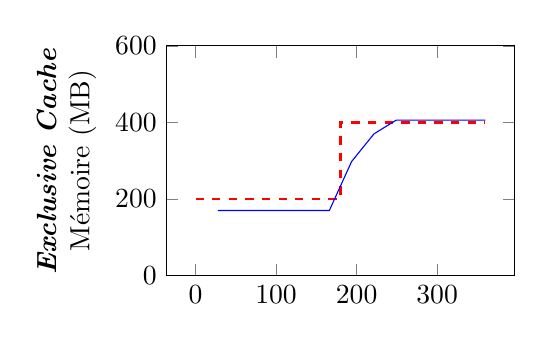
\begin{tikzpicture}
 \begin{axis}[
        height=4.5cm,
        width=6cm,
        %legend style={at={(0.5,1.45)},anchor=north,legend columns=-1},        
        ymax=600,
        ymin=0,
  %legend cell align=left, 
        ylabel near ticks,
        ylabel style={align=center}, 
        ylabel={\textbf{{\em Exclusive Cache}}\\Mémoire (MB)},
  ]%[name path=A] 
  \addplot [red,dashed,line width=1pt] coordinates {
    (0,200) (180,200) (180,400) (360,400)
  };  
   \addplot [blue] coordinates {
    (27.6923076923,170) (55.3846153846,170) (83.0769230769,170) (110.7692307692,170) (138.4615384615,170) (166.1538461538,170) (193.8461538461,298) (221.5384615384,370) (249.2307692307,406) (276.923076923,406) (304.6153846153,406) (332.3076923076,406) (359.9999999999,406)
  }; 
  %\legend{$W^o_{3}$,$W^e_{3}$}        
\end{axis}  
\end{tikzpicture} 
%%%%%%%%%%%%%%%%%%%%%%%%%%%%%%%%%%%%%%%%%%%%%%%%%%%%%
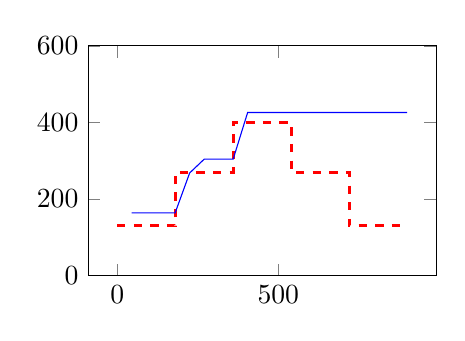
\begin{tikzpicture}
 \begin{axis}[
        height=4.5cm,
        width=6cm,
        %legend style={at={(0.5,1.45)},anchor=north,legend columns=-1},        
        ymax=600,
        ymin=0,
  %legend cell align=left, 
        ylabel near ticks,
  ]%[name path=A] 
  \addplot [red,dashed,line width=1pt] coordinates {
     (0,130) (180,130) (180,270) (360,270) (360,400) (540,400) (540,270) (720,270) (720,130) (900,130)  
  };
  \addplot [blue] coordinates {
     (45,164) (90,164) (135,164) (180,164) (225,268) (270,304) (315,304) (360,304) (405,426) (450,426) (495,426) (540,426) (585,426) (630,426) (675,426) (720,426) (765,426) (810,426) (855,426) (900,426)
  };  
  %\legend{$W^o_{5}$,$W^e_{5}$}         
 \end{axis}
\end{tikzpicture}

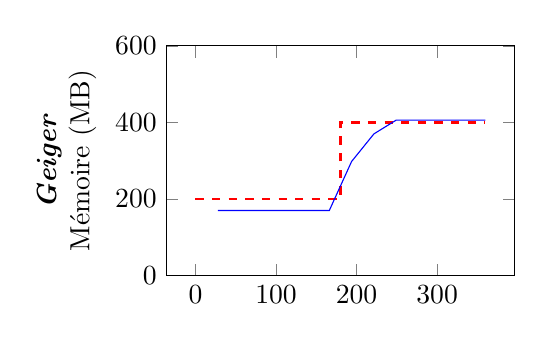
\begin{tikzpicture}
 \begin{axis}[
        height=4.5cm,
        width=6cm,
        %legend style={at={(0.5,1.45)}, anchor=north,legend columns=-1},        
        ymax=600,
        ymin=0,
  %legend cell align=left, 
        ylabel near ticks,
        ylabel style={align=center}, 
        ylabel={\textbf{{\em Geiger}}\\Mémoire (MB)},
  ]%[name path=A] 
  \addplot [red,dashed,line width=1pt] coordinates {
    (0,200) (180,200) (180,400) (360,400)
  };  
   \addplot [blue] coordinates {
    (27.6923076923,170) (55.3846153846,170) (83.0769230769,170) (110.7692307692,170) (138.4615384615,170) (166.1538461538,170) (193.8461538461,298) (221.5384615384,370) (249.2307692307,406) (276.923076923,406) (304.6153846153,406) (332.3076923076,406) (359.9999999999,406)
  }; 
  %\legend{$W^o_{3}$,$W^e_{3}$}        
\end{axis}  
\end{tikzpicture}  
%%%%%%%%%%%%%%%%%%%%%%%%%%%%%%%%%%%%%%%%%%%%%%%%%%%%%
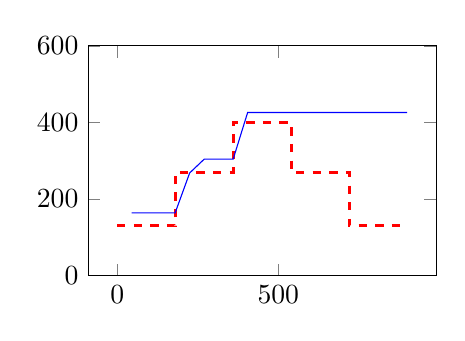
\begin{tikzpicture}
 \begin{axis}[
        height=4.5cm,
        width=6cm,
        %legend style={at={(0.5,1.45)},anchor=north,legend columns=-1},        
        ymax=600,
        ymin=0,
  %legend cell align=left, 
        %ylabel near ticks,
  ]%[name path=A] 
  \addplot [red,dashed,line width=1pt] coordinates {
     (0,130) (180,130) (180,270) (360,270) (360,400) (540,400) (540,270) (720,270) (720,130) (900,130)  
  };  
  \addplot [blue] coordinates {
     (45,164) (90,164) (135,164) (180,164) (225,268) (270,304) (315,304) (360,304) (405,426) (450,426) (495,426) (540,426) (585,426) (630,426) (675,426) (720,426) (765,426) (810,426) (855,426) (900,426)
  };  
  %\legend{$W^o_{5}$,$W^e_{5}$}         
 \end{axis}
\end{tikzpicture} 
 
\caption{Résultats d'évaluations des charges variables avec les techniques existantes. $W^o_{ss}$ : WSS escompté -- $W^e_{ss}$ WSS estimé}
\label{fig:studied_technique_ws_var}
\end{figure}